\documentclass[main.tex]{subfiles}

\begin{document} 
\begin{sloppypar}
\section{Simulation and Results}
\label{sec:newsimulation}
To evaluate the effectiveness of the proposed trajectory optimization framework, we conduct simulations for two representative tasks: static balance and walking. \\
\\
The analysis begins with an overview of key implementation details, focusing on the initialization of cost weights, time discretization parameters, and control bounds. These parameters define the structure of the optimization problem and facilitate the computation of feasible trajectories. Next, we outline the algorithm used to generate the desired reference trajectory for each task, establishing the target path for the robot’s motion. These trajectories serve as benchmarks, allowing us to assess the framework’s performance under different conditions.\\
\\
In this framework, contact states are represented using the set \{- , 0\}, where \{0\} indicates foot contact with the ground and \{-\} denotes a swing phase. Rather than using continuous time, trajectories are structured around these discrete contact phases, ensuring consistency in representation across both tasks. This approach allows for a more intuitive interpretation of contact dynamics and simplifies the integration of state transitions. \\
\\
With the reference trajectories defined, we proceed to analyze the simulation results by examining key components of the robot’s motion. First, we assess the CoM trajectories to determine how effectively the robot maintains stability and follows the intended path over time. Next, we compare the optimized state solutions with the reference trajectories at each contact step, providing insights into the effectiveness of the control strategy. Finally, we assess the contact wrenches, focusing on both translational and rotational forces to verify compliance with physical constraints and to evaluate the feasibility of the generated trajectories. \\
\paragraph{Implementation Overview}
Our work builds upon the framework provided in the IS - MPC Repository\footnote{\url{https://github.com/DIAG-Robotics-Lab/ismpc}}, which originally offers a comprehensive platform for simulating the HRP4 robot, including the dynamics model and control architecture. We have adapted and integrated our own implementation of the dynamics, trajectory optimization problem, and reference trajectory generation algorithm into the original repository. This integration enables the simulation of the HRP4 robot performing both the still and walking tasks, allowing us to assess the robot’s performance under our modified control and optimization framework.
\subsection{Implementation Details}
Implementing the proposed SBCD model involves requires careful consideration of parameter selection, initialization, and optimization for both static and walking scenarios. Given that the parameter configuration is largely consistent across both scenarios, a unified framework is presented, with task-specific distinctions clearly specified where relevant.
\paragraph{Parameter Initialization and Dynamics} The implementation leverages the IPOPT solver from the CasADi optimization framework to compute optimal trajectories based on the SBCD model. Both static and walking tasks are characterized by a shared set of parameters governing state initialization, dynamics, and control inputs. These parameters are systematically structured, allowing for easy adaptation between the two tasks. For both scenarios, the robot’s state is initialized with the Center of Mass positioned at a predefined reference point, with neutral feet orientations. Velocity initialization, however, is task-dependent. In the static scenario, CoM velocity is set to zero, serving as a baseline for assessing stationary behavior under SBCD control. In contrast, the walking task initialized the CoM velocity to [0, -0.07, 0]  (m/s), simulating an initial oscillation to the right. \\ 
\\
Before delving into the parameter values, Table \ref{tab:weight_states} outlines the specific weight configuration applied to some state components. While most parameters remain consistent, the weight for the velocity component differs between the two tasks: for the static task, it is set to 100, emphasizing minimal movement, whereas for the walking task, it is reduced to 1 to allow for more dynamic motion. For all other state components and control inputs, detailed in Eq. \eqref{eq:state_input}, weights are uniformly initialized to 1.
\begin{table}[h!]
    \centering
    \begin{tabular}{lcccccc}
    \toprule
    & $p_y$ & $p_z$ & $v_k$ & $L_k$ & $P_{L,k}$ & $Q_{L,k}$ \\
    \midrule
    Static & 500 & 500 & 100 & 1 & 100 & 0.0001 \\
    Walking & 500 & 500 & 1 & 1 & 100 & 0.0001 \\
    \bottomrule
    \end{tabular}
    \caption{Weight configuration for state components - Still and Walking Tasks}
    \label{tab:weight_states}
\end{table}
\paragraph{Optimization Framework} The optimization framework is designed to effectively handle contact-dependent dynamics by parameterizing state and control inputs for each contact phase. To achieve this, SBCD-based dynamics formulations are employed, enabling efficient computation of CoM trajectories and contact forces. This structured approach effectively manages transitions between single and double support phases during walking tasks.\\
\\
A crucial aspect of the optimization setup is the configuration of parameters that govern the behavior of both static and walking tasks. As illustrated in Table \ref{tab:optimization_params}, these parameters include the complementarity weight ($w_{compl}$), friction coefficients ($\mu$ and $\mu_z$), and phase duration limits ($\tau_{min}$ and $\tau_{max}$). Carefully setting these values ensures that the optimization framework remains grounded within the physical constraints of the robot’s actuators and the environmental interactions, striking a balance between control fidelity and physical feasibility.
\begin{table}[h!]
    \centering
    \begin{tabular}{lccccc}
        \toprule
        & $w_{compl}$ & $\mu$ & $\mu_z$ & $\tau_{max}$ & $\tau_{min}$ \\
        \midrule 
        Weight & 1000 & 0.5 & 0.6 & 10 & 0.4 \\
        \bottomrule
    \end{tabular}
    \caption{Optimization parameters - Still and Walking Tasks}
    \label{tab:optimization_params}
\end{table}
\\
\\
\subsection{Still Task}  
The objective of the still task is to keep the robot stationary, preserving its initial configuration throughout the entire trajectory. As indicated in Table~\ref{tab:stilltask}, the contact sequence ensures that both feet remain grounded, establishing a condition of complete stability without locomotion.
\begin{table}[h!]
    \centering
    \begin{tabular}{|c|c|c|c|}
    \hline
    Task & N & Foot & Contact Sequence \\
    \hline
    Still & 4 & Right & 0000 \\
    & & Left & 0000 \\
    \hline
    \end{tabular}
    \caption{Contact sequence - Still Task}
    \label{tab:stilltask}
\end{table}
\paragraph{Reference Trajectory Generation}  
The still task algorithm (Algorithm~\ref{alg:stilltask}) generates reference state and control trajectories aimed at preserving the robot’s initial configuration throughout the task duration. By maintaining constant CoM position, orientation, and feet positions, the algorithm ensures that the robot remains stationary, counteracting gravitational forces through ground reaction forces. The algorithm begins by initializing the state \( X_{ref} \) and control \( U_{ref} \) matrices to zero. At each timestep, the CoM and feet positions are held fixed while ground reaction forces are adjusted to stabilize the robot against gravitational effects. This approach effectively prevents any unintended motion, maintaining the initial configuration without deviations.\\
\begin{algorithm}[H]
\caption{Reference Trajectory Still Task Generation}
\label{alg:stilltask}
\begin{algorithmic}[1]
\State Initialize state matrix \( X_{ref} \in \mathbb{R}^{28 \times N} \) and control matrix \( U_{ref} \in \mathbb{R}^{27 \times (N-1)} \) to zero
\State Set initial CoM/feet position and orientation and $t_0 \gets 0$ in \( X_{ref}(0) \)
\For{\( k = 0 \) to \( N-1 \)}
    \State Set \( X_{ref}(k+1) \) as a copy of the current state \( X_{ref}(k) \)
    \State Set desired phase\_duration $\tau_k$ and contact force gains $\lambda_k$ in  \( U{ref}(k) \)
    \State Update \( X_{ref}(k+1) \) with $t_{k+1} \gets t_k + \tau_k$
\EndFor
\State \Return \( X_{ref}, U_{ref} \)
\end{algorithmic}
\end{algorithm}
\paragraph{Simulation Results}
Visual results are presented to illustrate the outcomes of the still task simulation, providing a comprehensive view of the system’s behavior under stationary conditions.\\
\\
The plots in Fig.\ref{fig:com_still} illustrate the CoM evolution during the still task. The \( x \) component displays slight horizontal drift, likely due to adjustments in ground reaction forces, while the \( y \) component briefly dips before stabilizing, indicating corrective measures to maintain balance. The \( z \) component initially drops and then recovers, reflecting gravitational compensation. Despite these fluctuations, the CoM remains largely consistent, demonstrating effective stabilization. \\
\begin{figure}[H]
    \centering
    \begin{subfigure}[b]{0.32\textwidth}
        \centering
        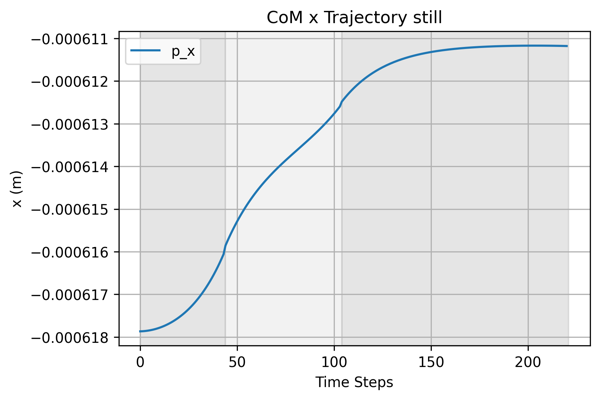
\includegraphics[width=\textwidth]{C:/Users/giuse/OneDrive/Desktop/GITHUB PROJECTS/AMR-FP1/centroidal_dyn-main/plots/CoM x Trajectory still.png}
        \caption{CoM x component}
        \label{fig:com_x_still}
    \end{subfigure}
    \hfill
    \begin{subfigure}[b]{0.32\textwidth}
        \centering
        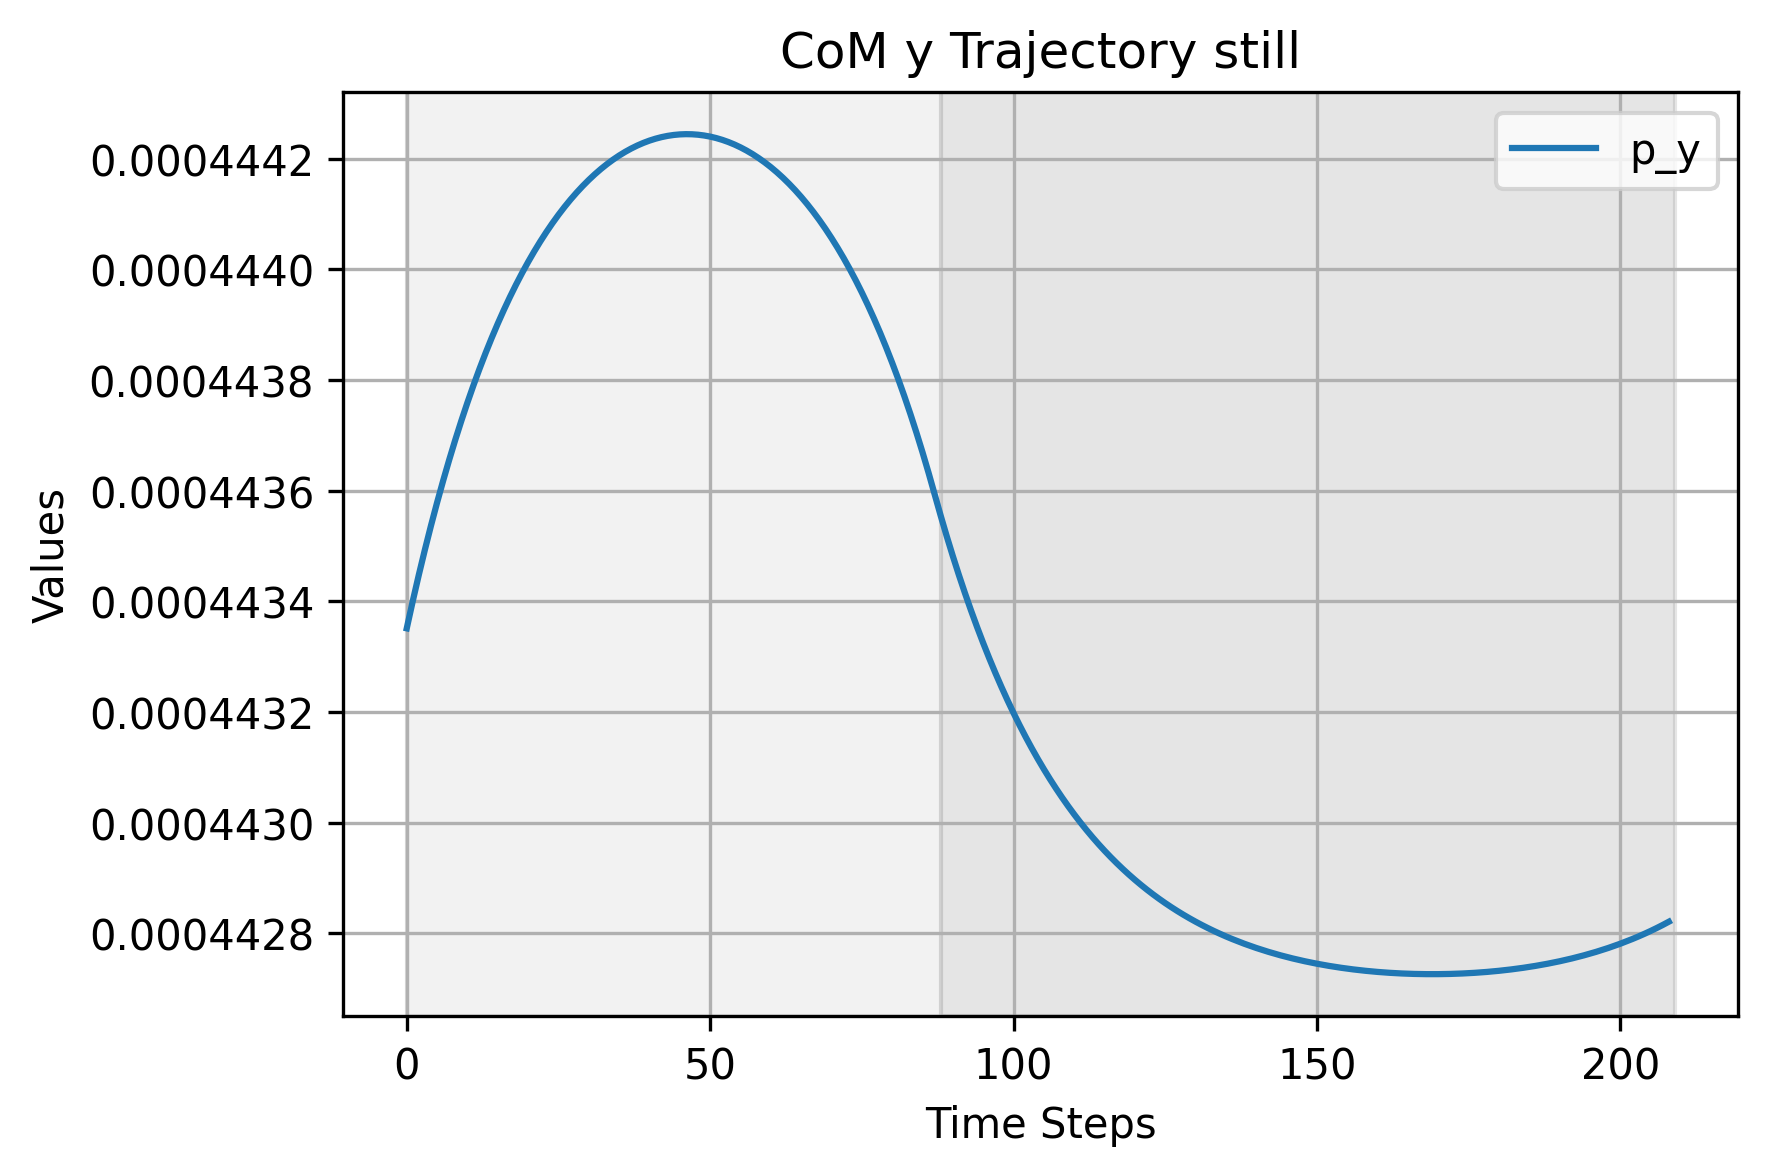
\includegraphics[width=\textwidth]{C:/Users/giuse/OneDrive/Desktop/GITHUB PROJECTS/AMR-FP1/centroidal_dyn-main/plots/CoM y Trajectory still.png}
        \caption{CoM y component}
        \label{fig:com_y_still}
    \end{subfigure}
    \hfill
    \begin{subfigure}[b]{0.32\textwidth}
        \centering
        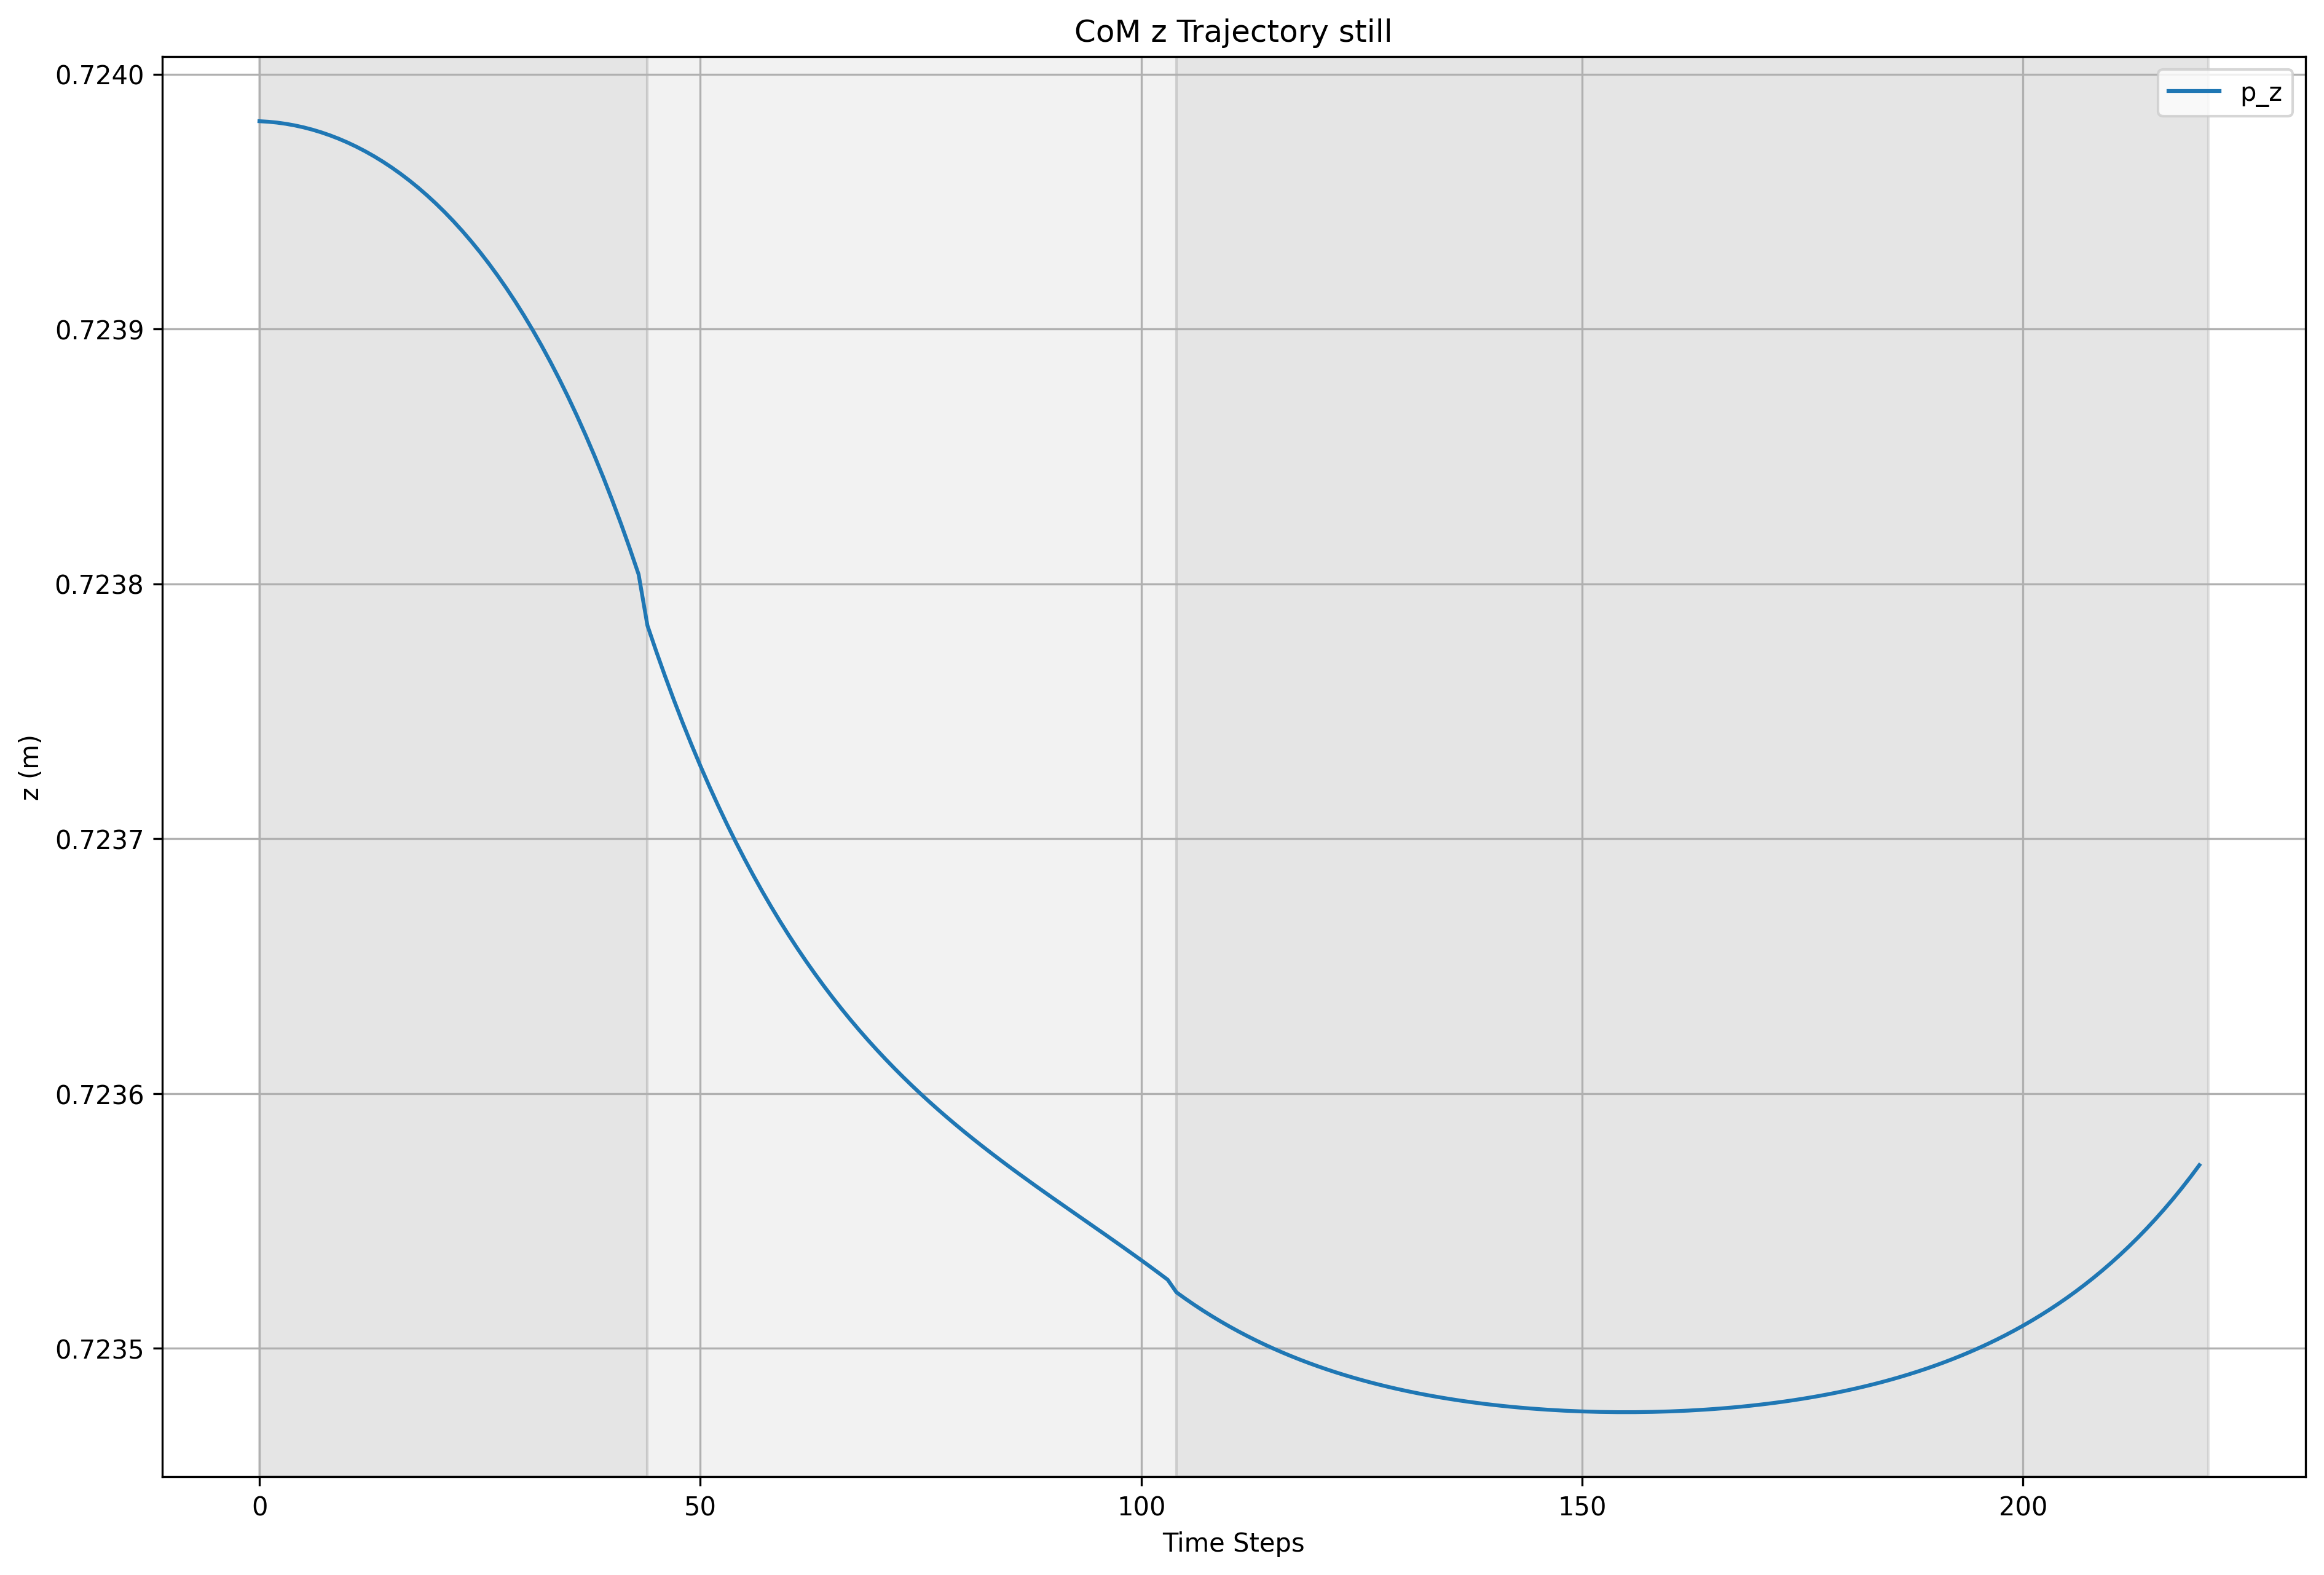
\includegraphics[width=\textwidth]{C:/Users/giuse/OneDrive/Desktop/GITHUB PROJECTS/AMR-FP1/centroidal_dyn-main/plots/CoM z Trajectory still.png}
        \caption{CoM z component}
        \label{fig:com_z_still}
    \end{subfigure}
    \caption{Evolution of CoM Position - Still Task}
    \label{fig:com_still}
\end{figure}
Fig.\ref{fig:three_still} shows the evolution of feet positions along the z-axis, CoM velocity, and angular momentum during the still task. The feet positions in Fig. \ref{fig:feet_z_still} remain nearly constant, indicating minimal vertical motion. In Fig. \ref{fig:com_velocity_still}, slight oscillations in the $y$ and $z$ velocity components suggest minor corrective actions to maintain stability. The angular momentum in Fig. \ref{fig:angular_momentum_still} exhibits some oscillations in the $L_y$ component, suggesting subtle internal dynamics. The $L_x$ component displays smaller, gradually decaying oscillations, indicating mild corrective adjustments. Meanwhile, the $L_z$ component remains steady at zero, reflecting a stable and balanced configuration around the $z$ - axis. 
\begin{figure}[htbp]
    \centering
    \begin{subfigure}[b]{0.32\textwidth}
        \centering
        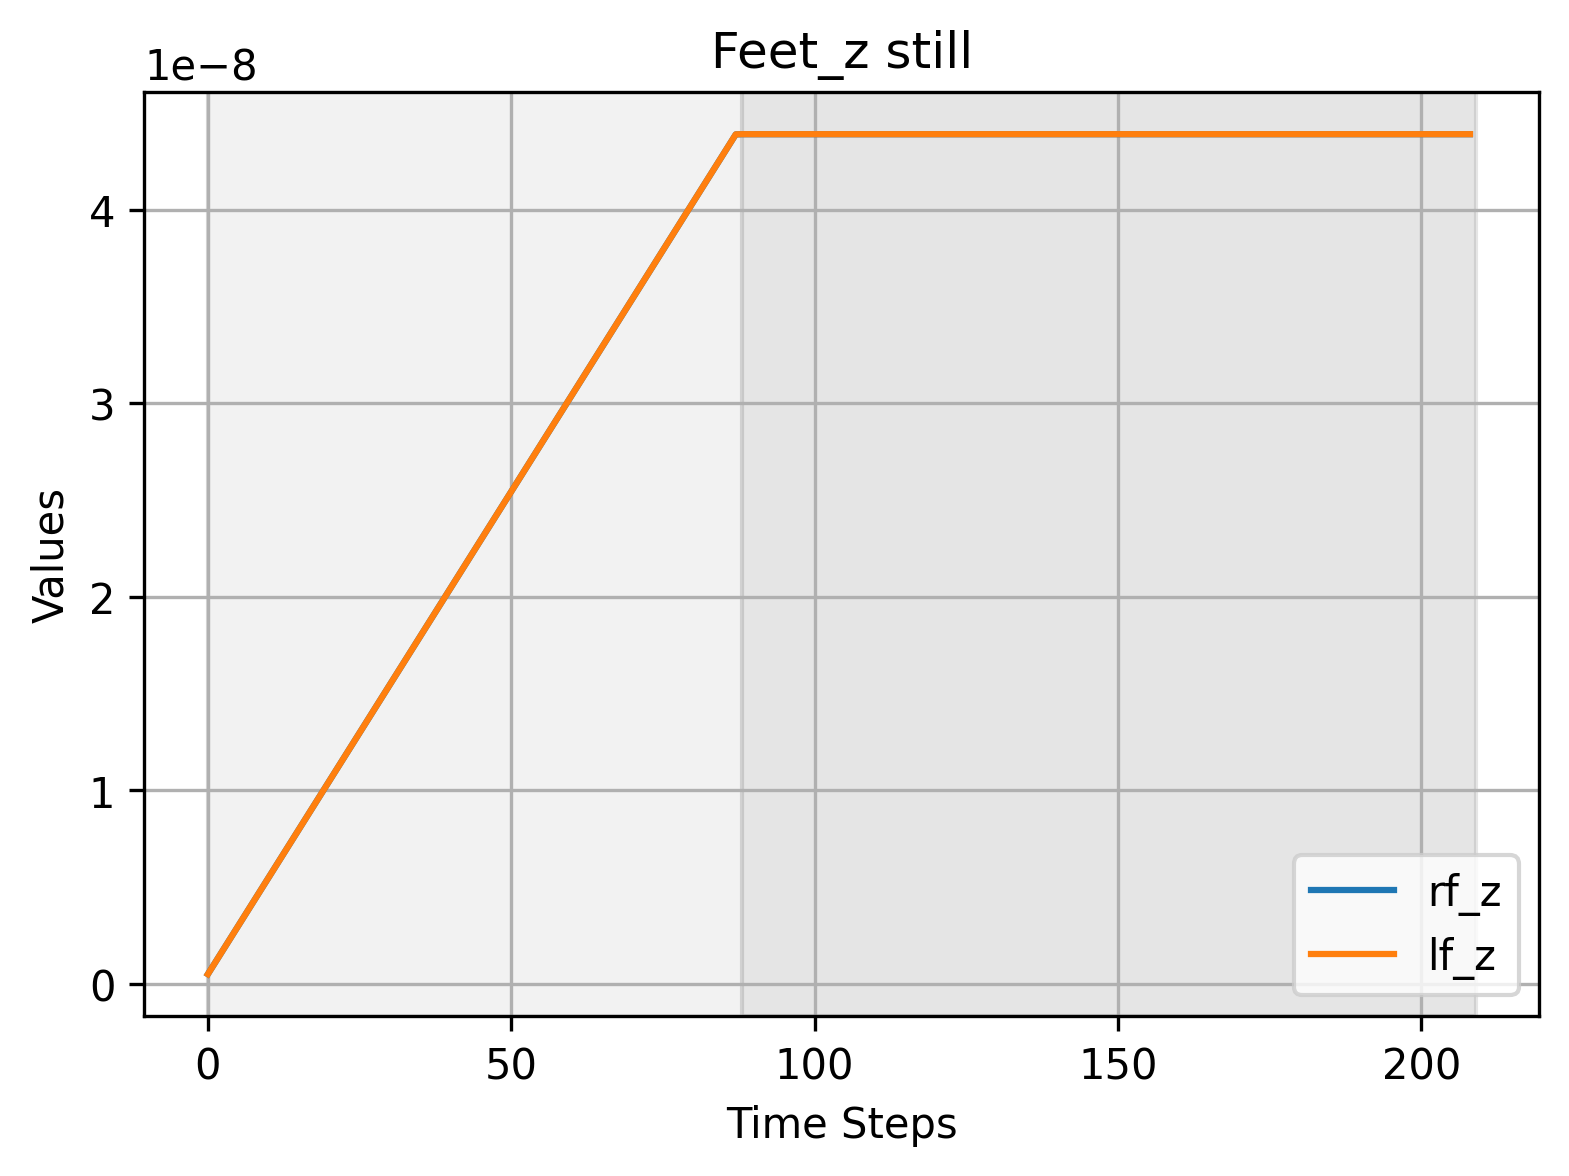
\includegraphics[width=\textwidth]{C:/Users/giuse/OneDrive/Desktop/GITHUB PROJECTS/AMR-FP1/centroidal_dyn-main/plots/Feet_z still.png}
        \caption{Feet along z axis}
        \label{fig:feet_z_still}
    \end{subfigure}
    \hfill
    \begin{subfigure}[b]{0.32\textwidth}
        \centering
        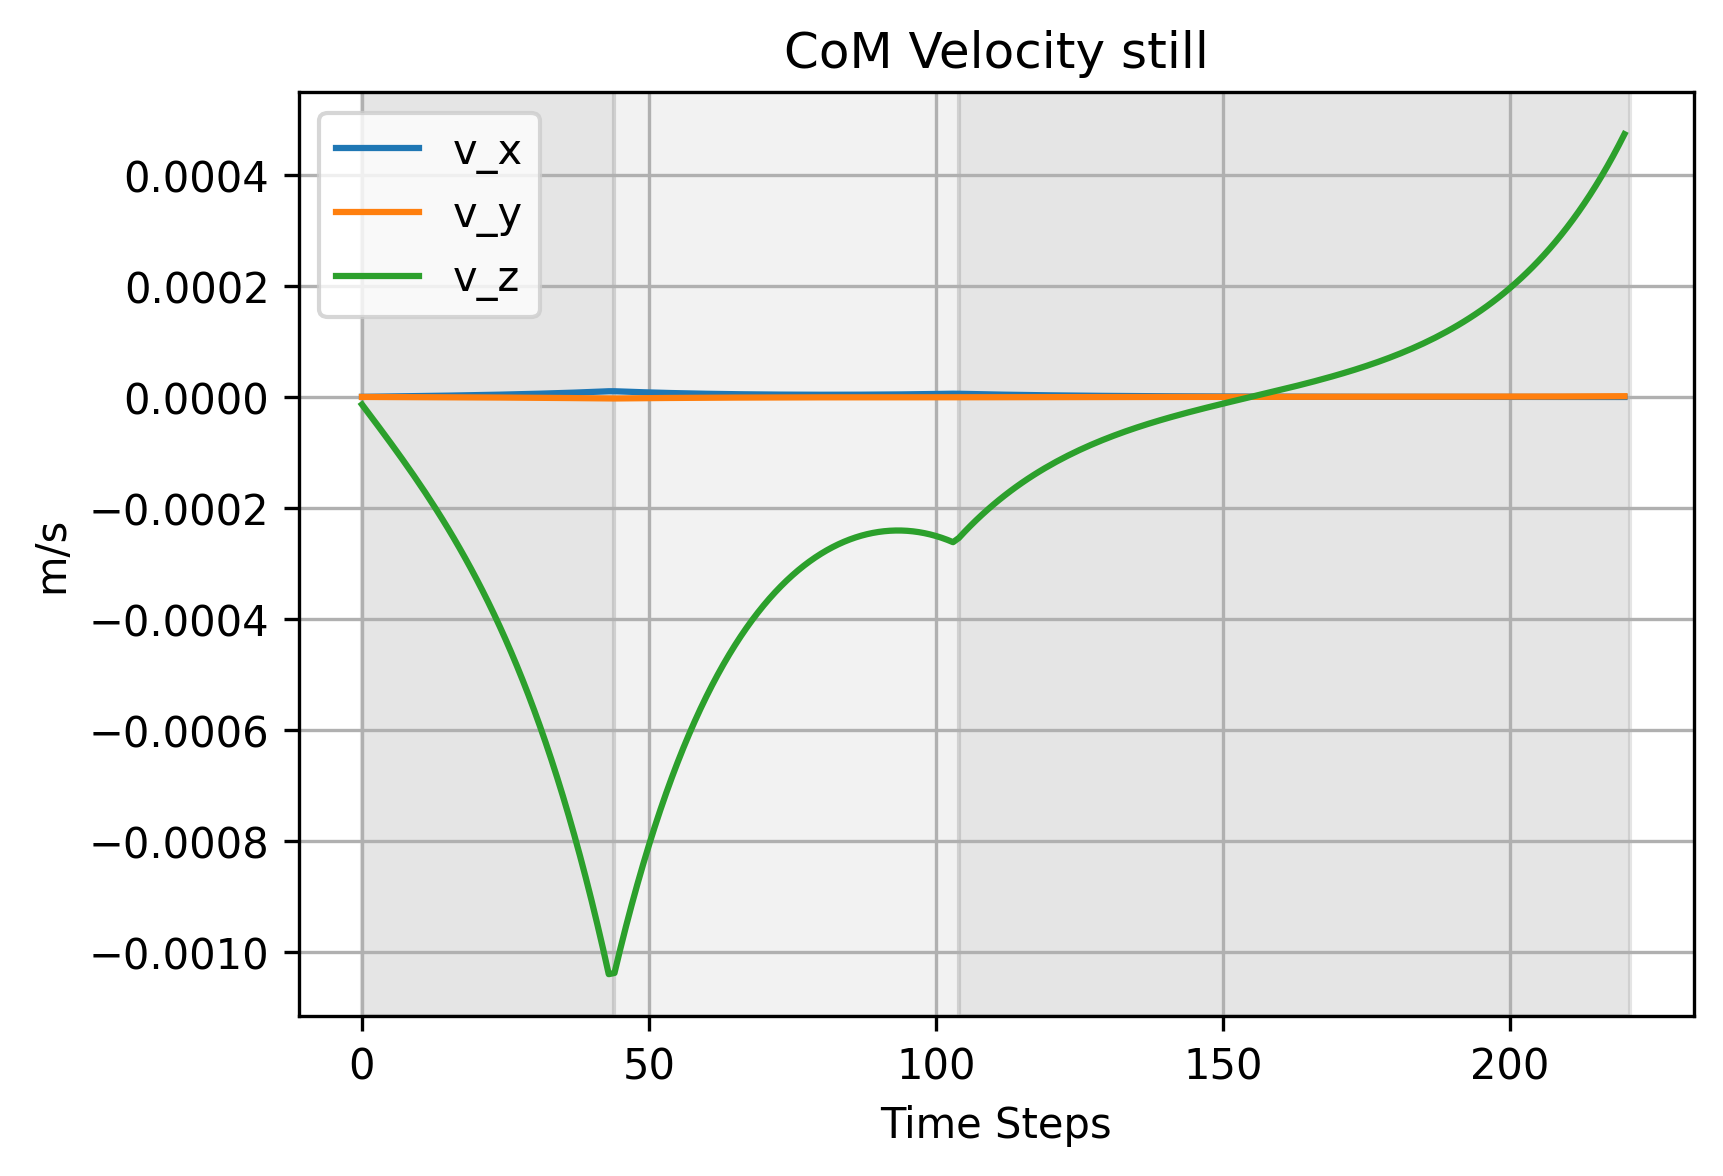
\includegraphics[width=\textwidth]{C:/Users/giuse/OneDrive/Desktop/GITHUB PROJECTS/AMR-FP1/centroidal_dyn-main/plots/CoM Velocity still.png}
        \caption{CoM Velocity}
        \label{fig:com_velocity_still}
    \end{subfigure}
    \hfill
    \begin{subfigure}[b]{0.32\textwidth}
        \centering
        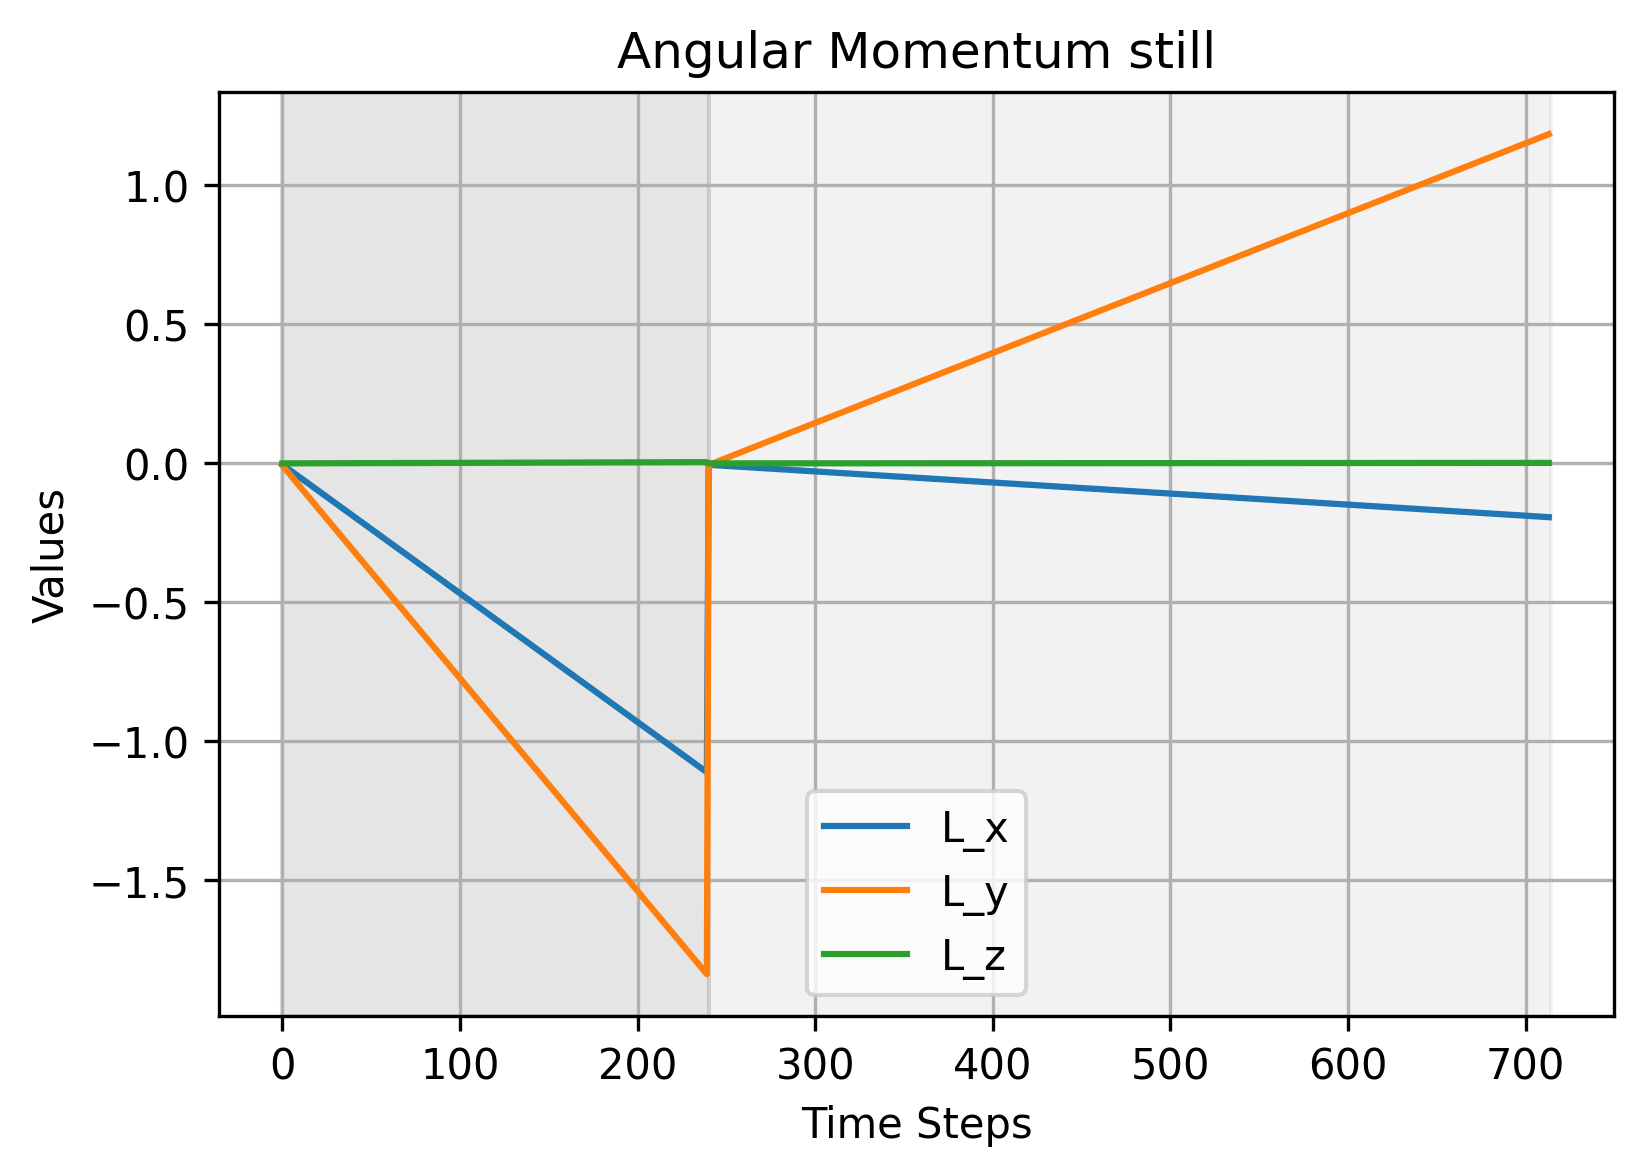
\includegraphics[width=\textwidth]{C:/Users/giuse/OneDrive/Desktop/GITHUB PROJECTS/AMR-FP1/centroidal_dyn-main/plots/Angular Momentum still.png}
        \caption{Angular Momentum}
        \label{fig:angular_momentum_still}
    \end{subfigure}
    \caption{Feet, Com Velocity and Angular Momentum - Still Task}
    \label{fig:three_still}
\end{figure}
\newpage
In Fig. \ref{fig:comparison_still} , the comparison between the reference and optimized trajectories for the still task is presented. The CoM position remains largely aligned with the reference values, with slight deviations observed primarily in the $x$ and $z$ components, reflecting minor adjustments to maintain stability. CoM velocity remains close to zero, consistent with the stationary objective, though minor oscillations indicate corrective actions against gravitational forces. Angular momentum closely follows the reference values across all components, inidicating that the system remains effectively stationary with minimal rotational adjustments. Feet positions and velocities remain effectively constant, confirming that the feet maintain their initial stance without significant movement. Overall, the optimized trajectories exhibit minimal divergence from the reference, indicating effective stabilization while accounting for minor corrections.
\begin{figure}[htbp]
    \centering
    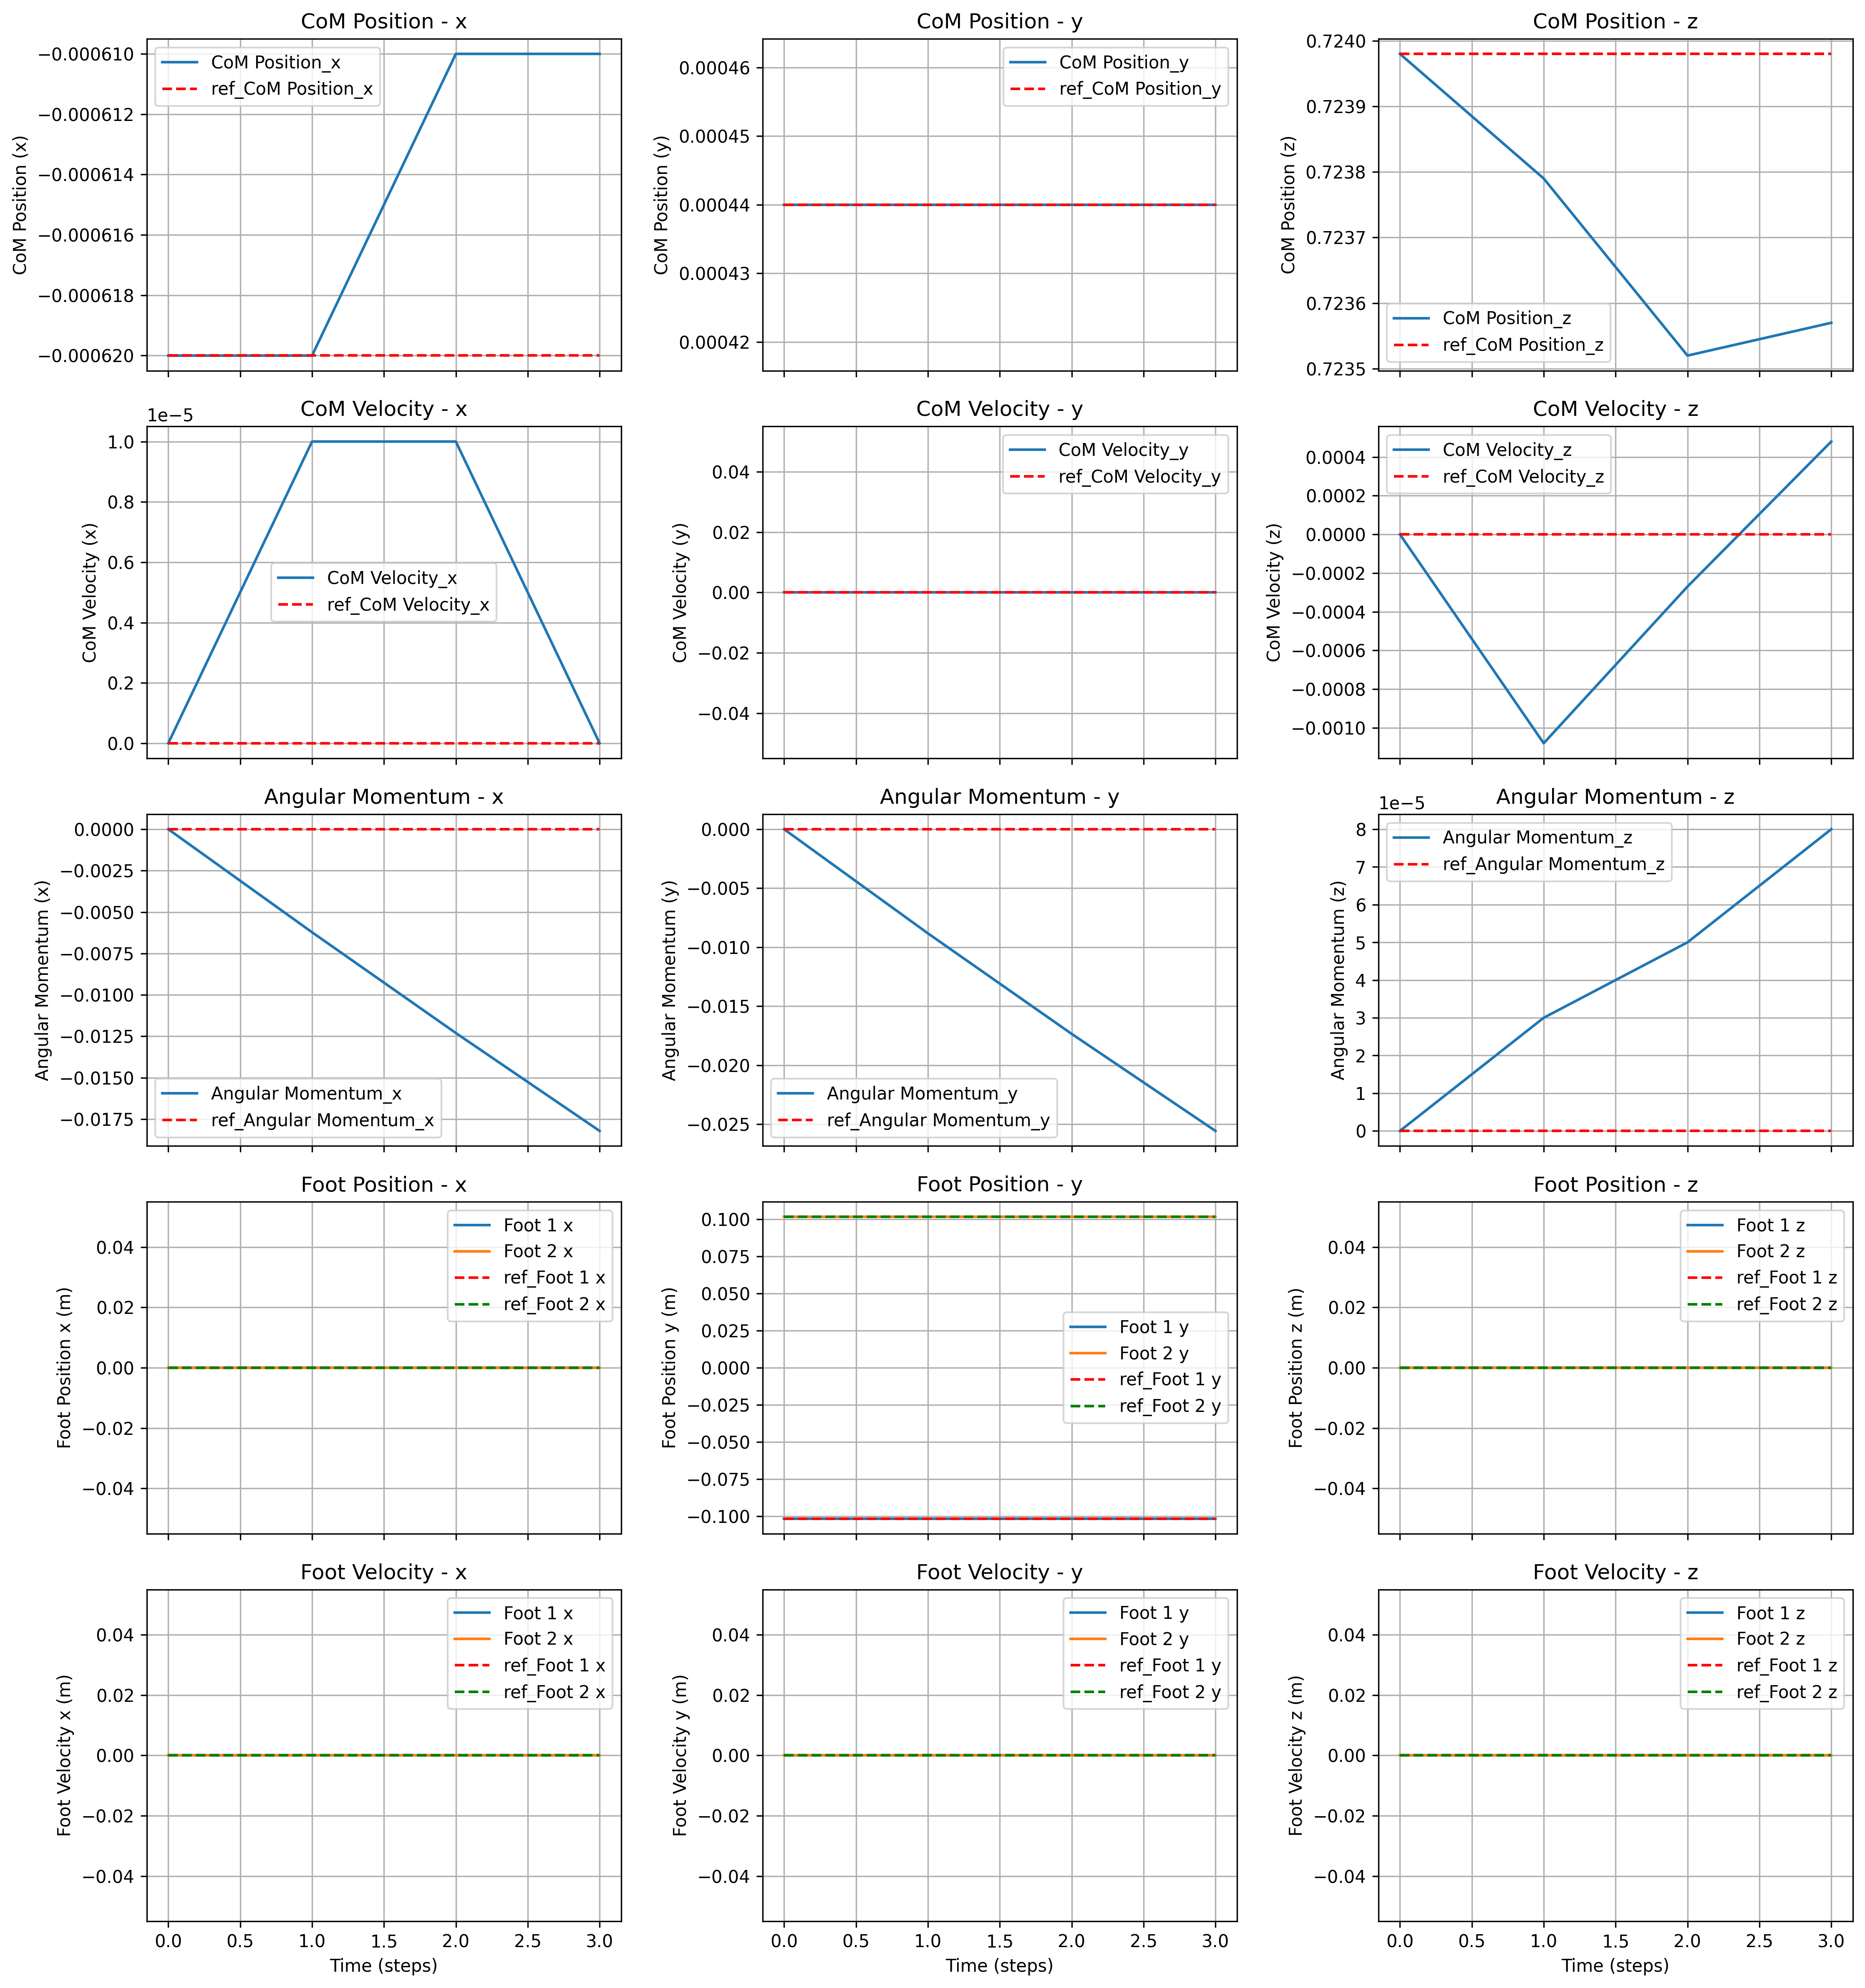
\includegraphics[width=0.8\textwidth]{C:/Users/giuse/OneDrive/Desktop/GITHUB PROJECTS/AMR-FP1/centroidal_dyn-main/plots/contact_x_still.png}
    \caption{Trajectory vs Reference - Still Task}
    \label{fig:comparison_still}
\end{figure}
\\
\\
Another key aspect of the dynamics involves the contact wrenches, which represent the mechanical forces and moments applied by contact points, such as the feet, on the robot or vice versa. To maintain dynamic balance, the reaction force along the $z$-axis must counteract the gravitational force acting on the robot’s mass. The contact forces from the environment on both feet are summarized in Table \ref{tab:forces_still}. As indicated, when both feet remain grounded, the gravitational force is evenly distributed between the left and right foot, ensuring stability. \\
\begin{table}[H]
    \centering
    \renewcommand{\arraystretch}{1.2}
    \resizebox{\textwidth}{!}{
        \begin{tabular}{c|c|c|c|c}
            \hline
            Interval & Right Foot (x,y,z) & Left Foot (x,y,z) & $\Sigma L_k$ & Sum Forces (x,y,z) \\
            \hline
            0 & (0.000059, 9.53808, 49.0403) & (0.000080, -9.53812, 49.046) & (0, 0) & (0.000139, -0.000038, 98.0863) \\
            1 & (-0.000233, 9.53903, 49.070) & (-0.000211, -9.53891, 49.0757) & (0, 0) & (-0.000444, 0.000127, 98.1457) \\
            2 & (-0.000143, 9.53922, 49.0531) & (-0.000121, -9.53918, 49.0587) & (0, 0) & (-0.000264, 0.000032, 98.1118) \\
            \hline
        \end{tabular}
    }
    \caption{Summary of Forces and Foot Positions per Interval - Still Task}
    \label{tab:forces_still}
\end{table}
\newpage
To conclude the analysis of the still task, Figures \ref{fig:contact_forces_still_right} and \ref{fig:contact_forces_still_left} illustrate the behavior of translational and rotational forces at the contact points for the right and left foot, respectively. Along the horizontal axes, translational forces in the \( x \) and \( y \) components remain near zero, indicating minimal lateral interaction with the ground. The vertical \( z \) component shows a pronounced peak, reflecting the compensation for gravitational forces with slight variations indicating minor adjustments. Rotational forces exhibit a more defined trend, particularly in the \( x \) and \( y \) components, with both displaying a gradual decline, suggesting a slight decrease in corrective torques over time. The \( z \) component shows a slight increase followed by a minor drop, with minor fluctuations that align the angular momentum behavior observed previously. 
\vspace*{2.5cm}
\begin{figure}[htbp]
    \centering
    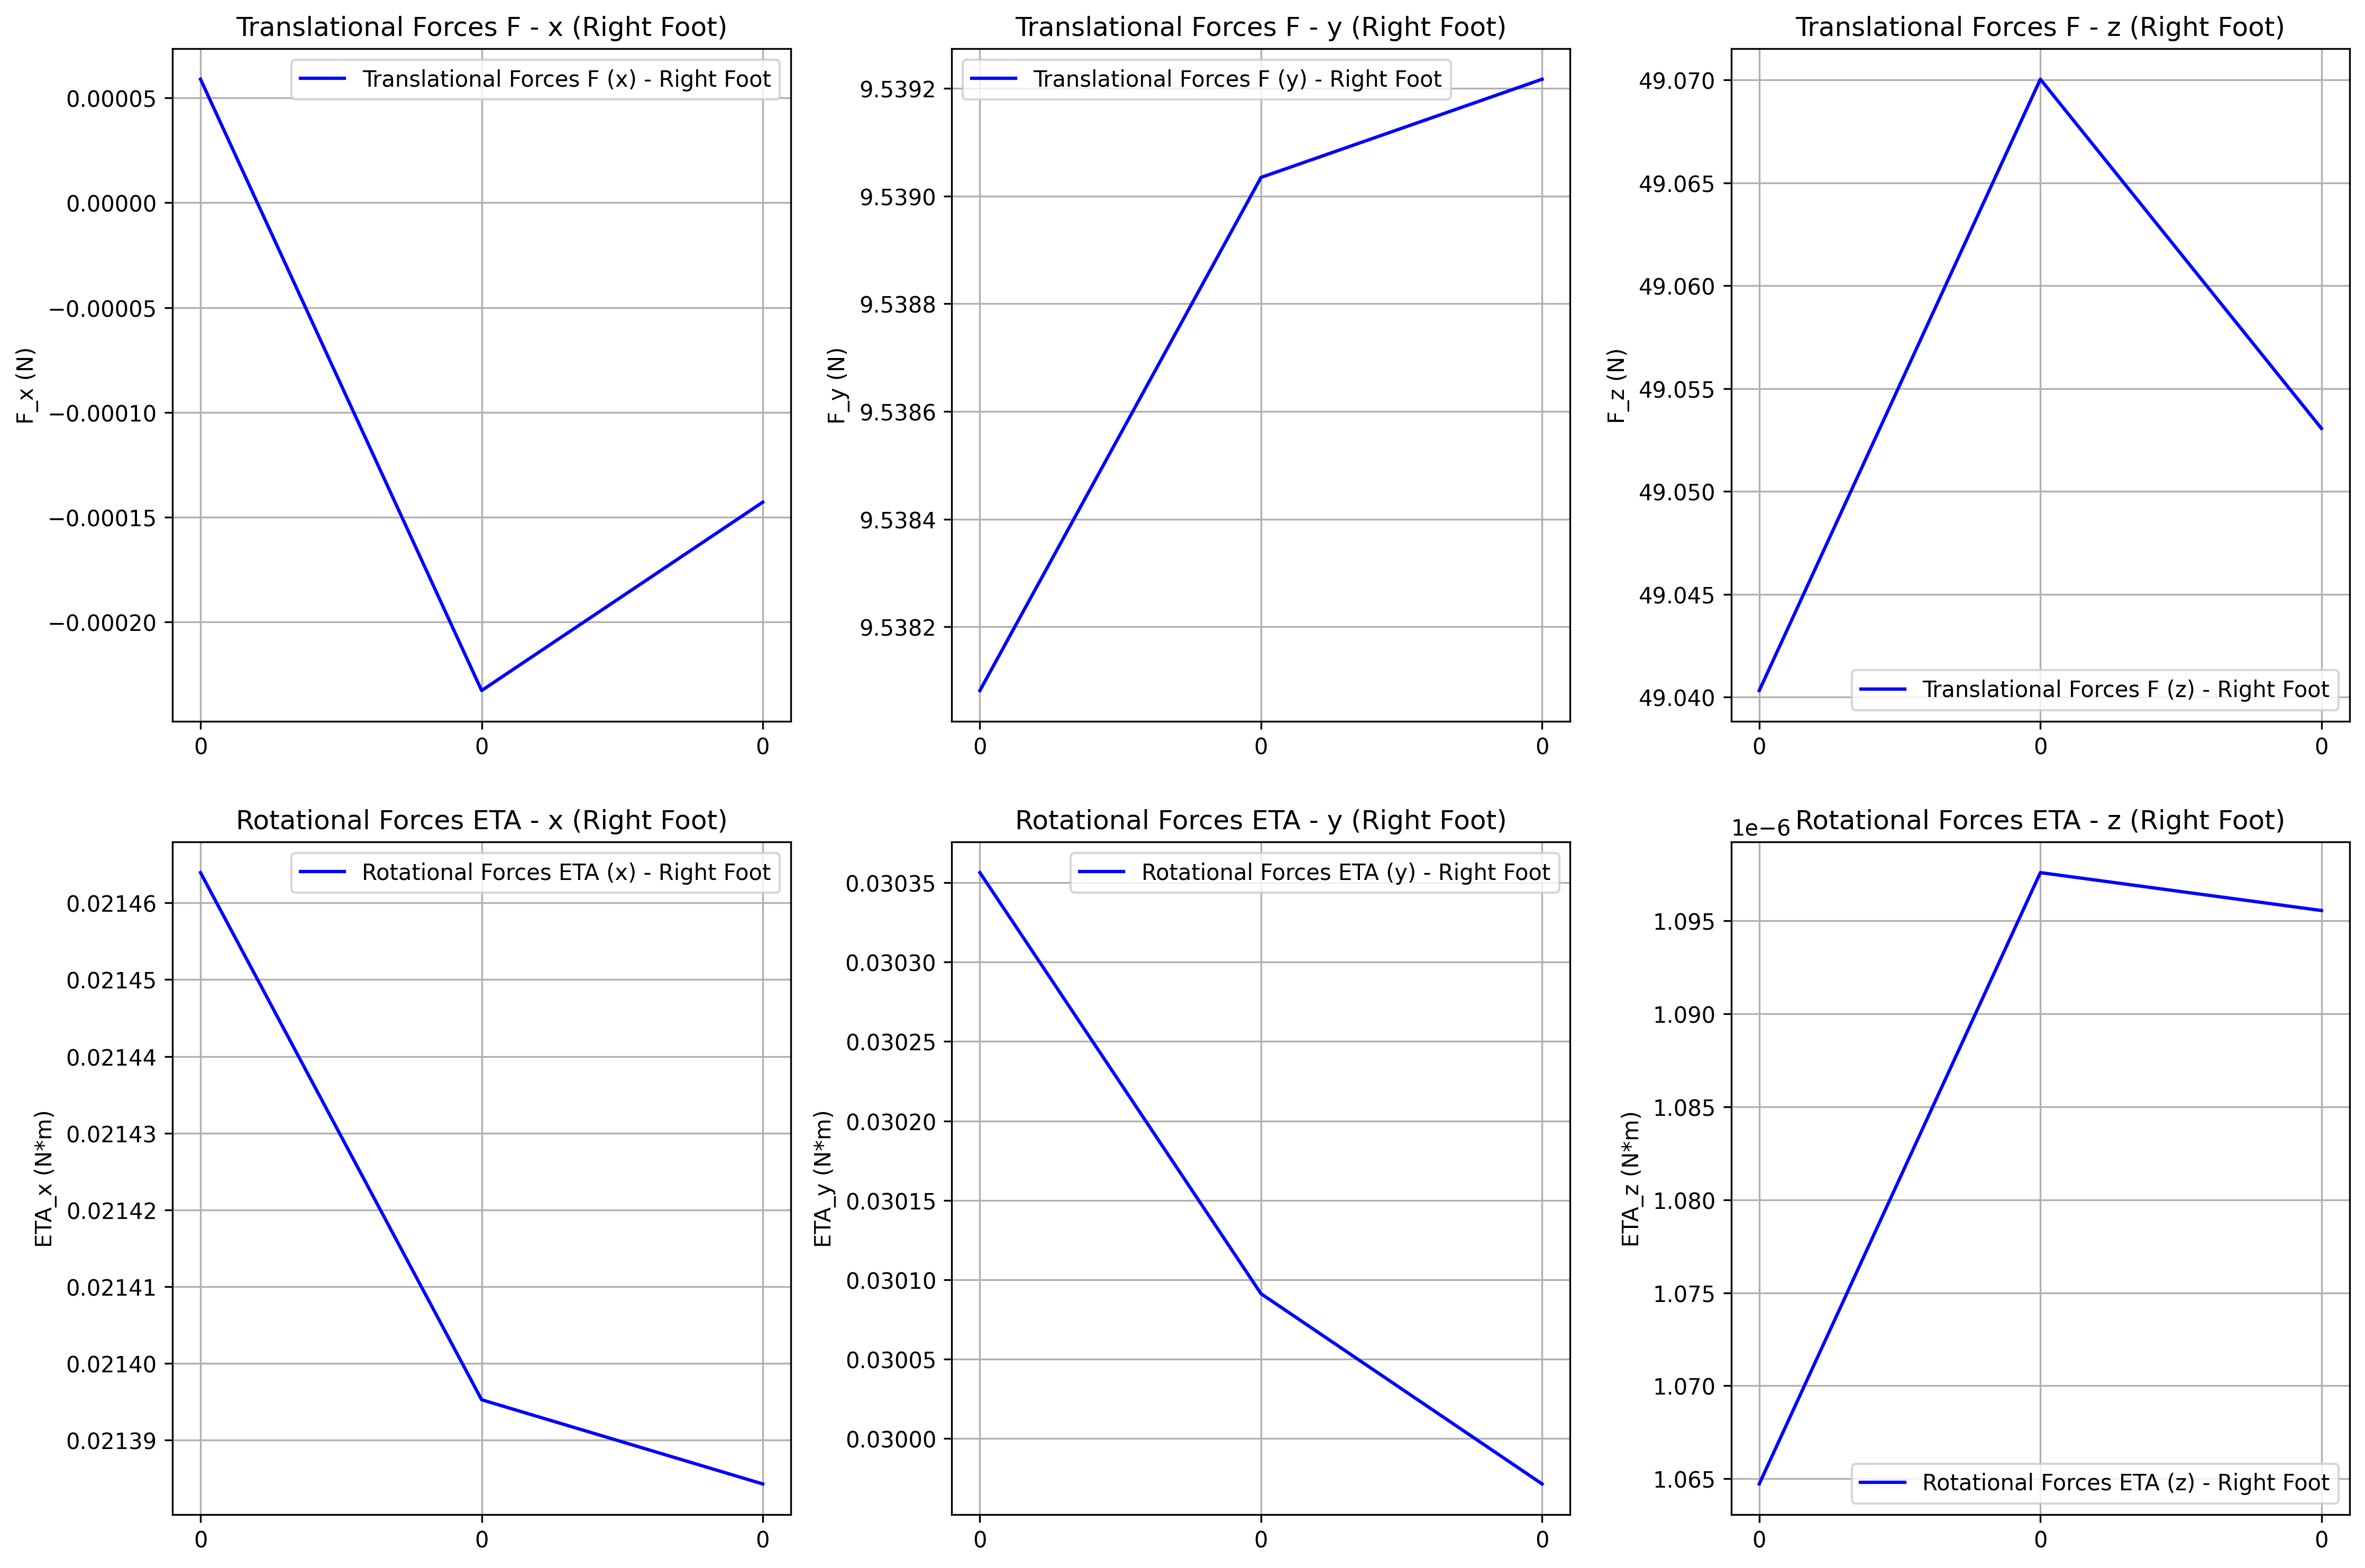
\includegraphics[width=0.8\textwidth]{C:/Users/giuse/OneDrive/Desktop/GITHUB PROJECTS/AMR-FP1/centroidal_dyn-main/plots/contact_forces_still_right.png}
    \caption{Translational and Rotational Forces Right Foot - Still Task}
    \label{fig:contact_forces_still_right}
\end{figure}
\begin{figure}[htbp]
    \centering
    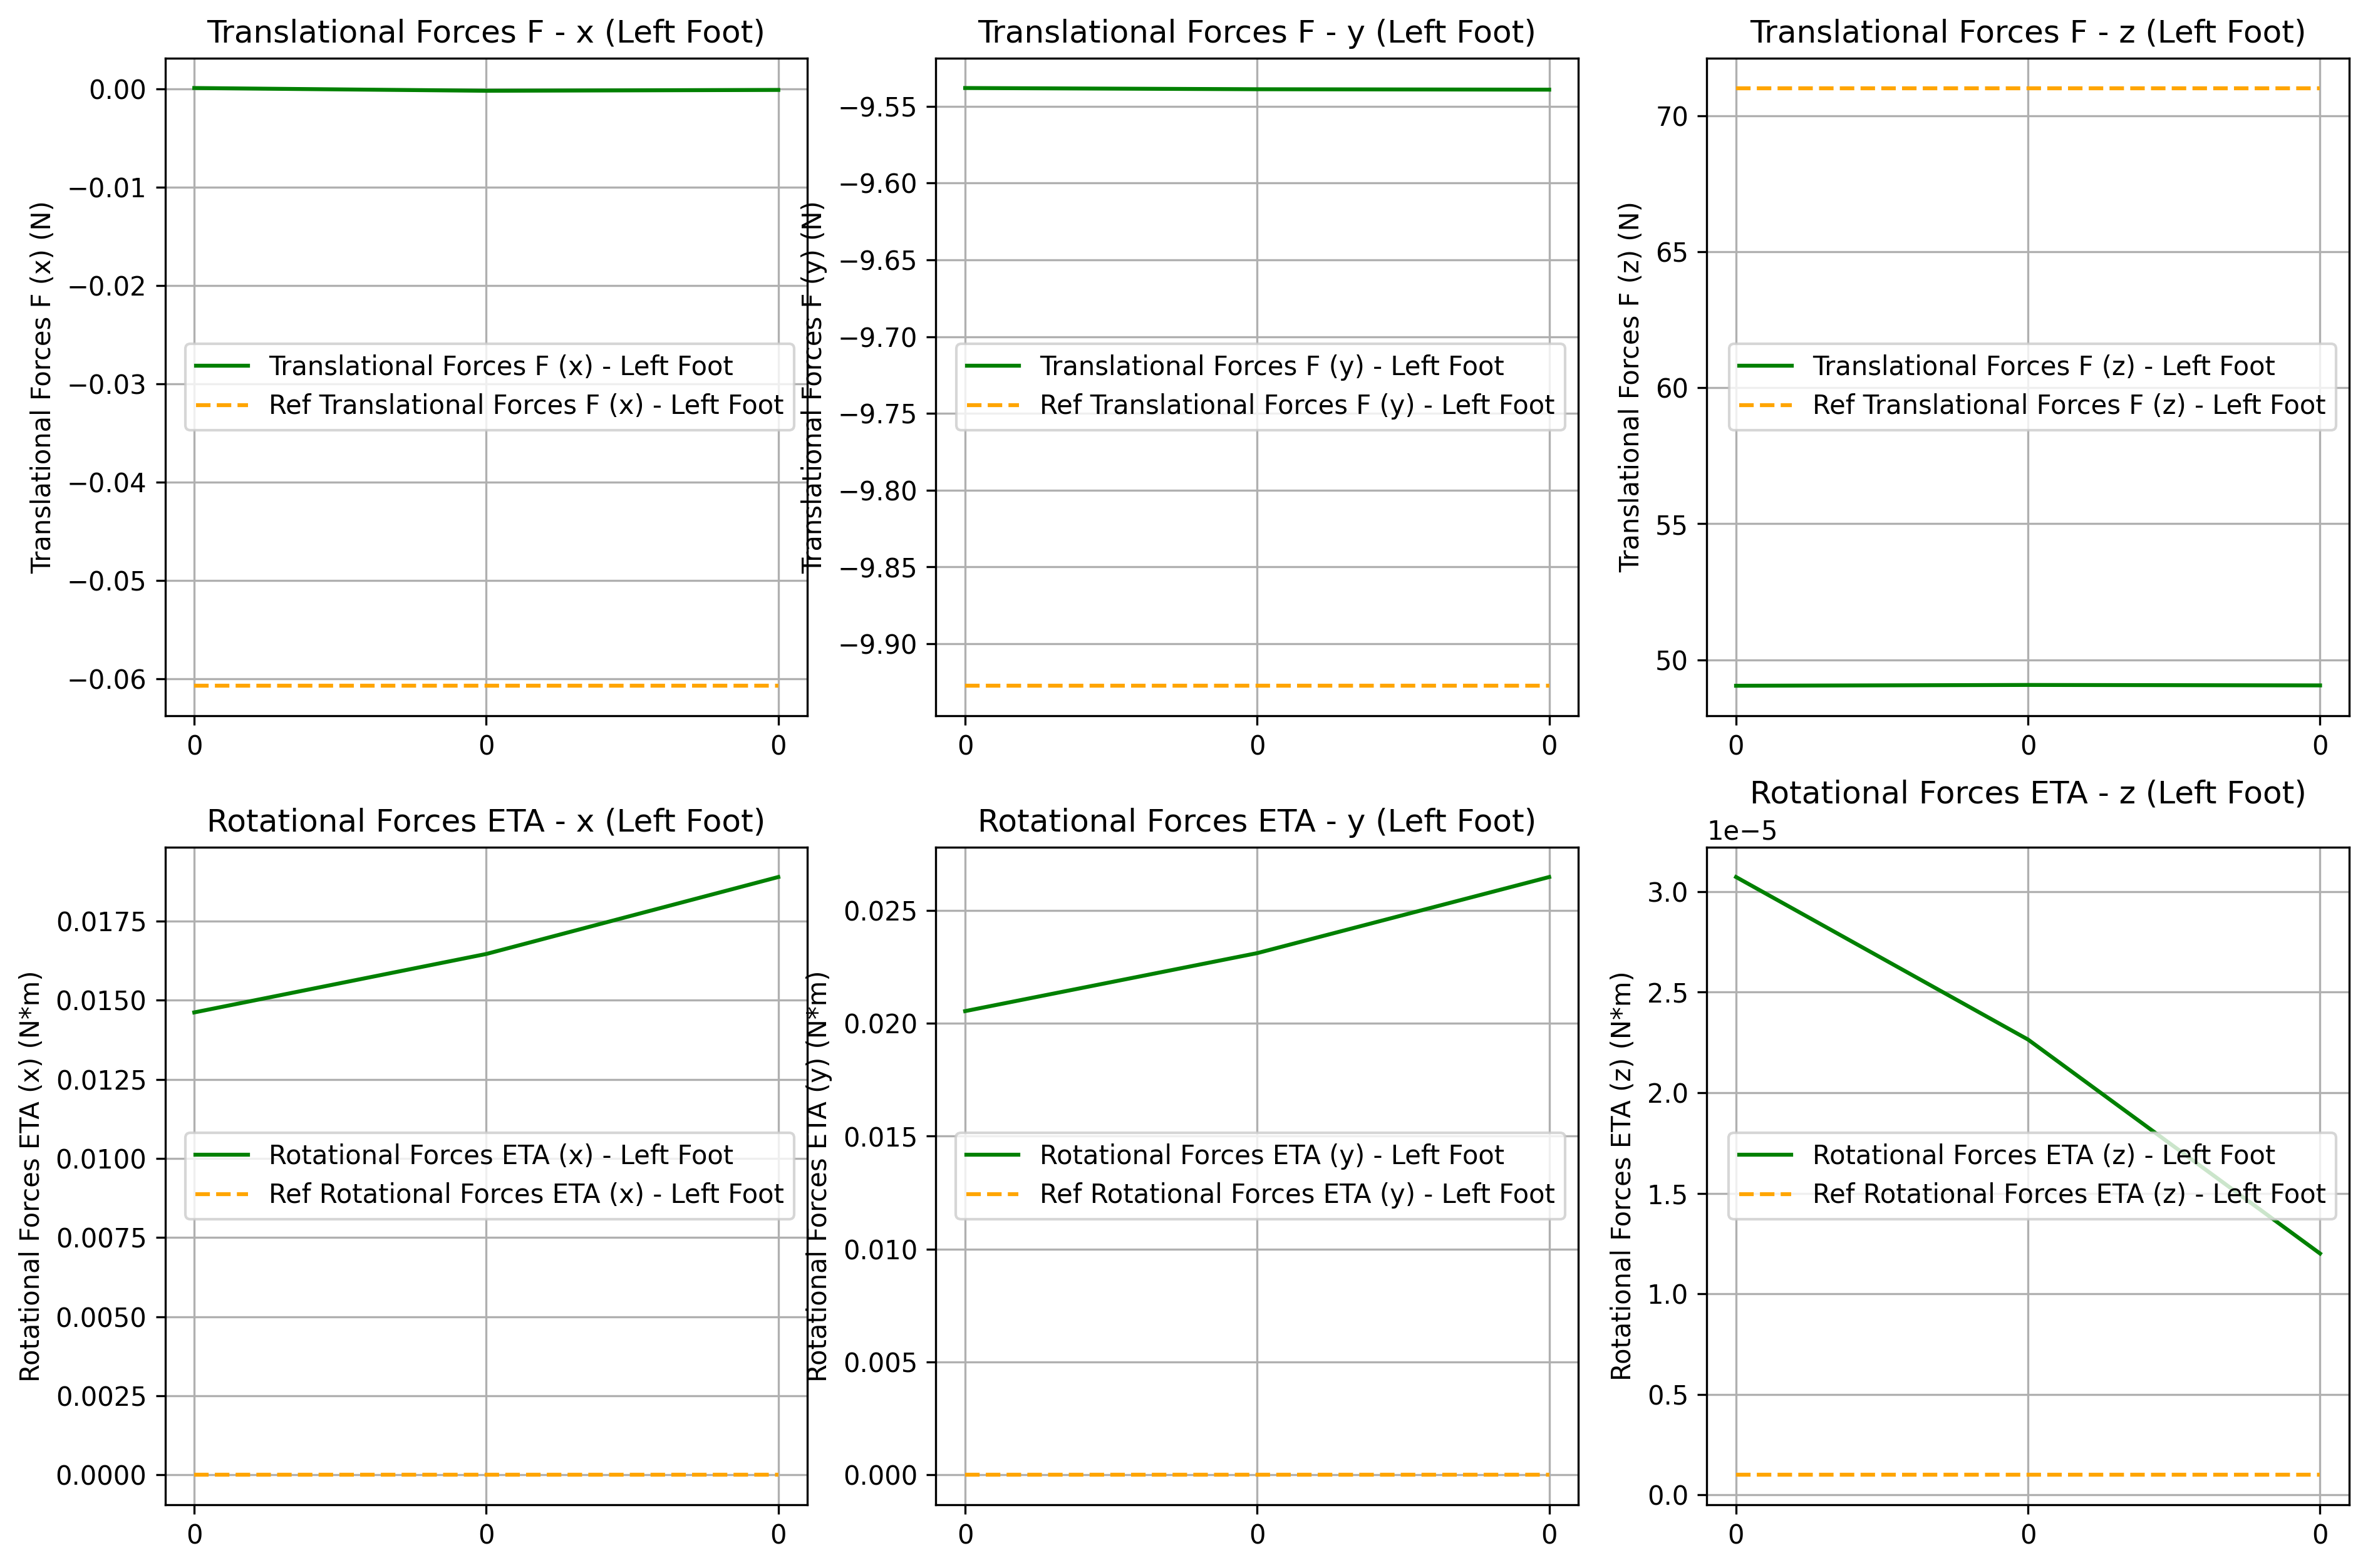
\includegraphics[width=0.8\textwidth]{C:/Users/giuse/OneDrive/Desktop/GITHUB PROJECTS/AMR-FP1/centroidal_dyn-main/plots/contact_forces_still_left.png}
    \caption{Translational and Rotational Forces Left Foot - Still Task}
    \label{fig:contact_forces_still_left}
\end{figure}
\newpage
\subsection{Walking Task}
The objective of the walking task is to simulate a natural walking pattern by coordinating the movements of the feet and the Center of Mass (CoM) through a sequence of double-support and single-support phases. During double-support phases, both feet remain in contact with the ground, maintaining stability. In single-support phases, one foot is lifted while the other remains grounded, allowing forward motion.
The CoM position update depends on the preceding phase. If the previous phase was double-support, the CoM remains stationary. Otherwise, it advances forward, ensuring consistent movement. The foot trajectory is constructed to mimic a natural step, extending the moving foot beyond the stationary one. The Z-coordinate of each foot follows a parabolic profile, ensuring smooth lift-off and descent.
The contact sequence for the walking task, presented in Table \ref{tab:walkingtask}, defines the alternating pattern of double and single-support phases, guiding the timing and transitions of each step.
\begin{table}[H]
    \centering
    \begin{tabular}{|c|c|c|c|}
        \hline
        Task & N & Foot & Contact Sequence \\
        \hline
        Walk & 24 & Right & 000-000-000-000-000-0 \\
             &    & Left  & 0-000-000-000-000-000 \\
        \hline
    \end{tabular}
    \caption{Contact sequence - Walking Task}
    \label{tab:walkingtask}
\end{table}
\paragraph{Reference Trajectory Generation}
The reference trajectory generation algorithm for the walking task is designed to compute state and control matrices that guide the robot's CoM and foot movements throughout the walking cycle. The algorithm initializes the robot's state, reads the contact sequence to identify double and single-support phases, and calculates the CoM and feet velocities based on the transition logic.
The CoM trajectory is computed by integrating velocities over the phase duration, while feet positions are updated based on contact states. The transition logic, detailed in Table \ref{tab:logic_walking}, specifies how velocities and displacements are adjusted for each phase.
\begin{algorithm}[H]
\caption{Reference Trajectory Generation - Walking Task}
\label{alg:walking_task}
\begin{algorithmic}[1]
\State Initialize state matrix \( X_{ref} \in \mathbb{R}^{28 \times (N)} \) and control matrix \( U_{ref} \in \mathbb{R}^{27 \times (N-1)} \) to zero
\State Set initial CoM/feet position and orientation and $t_0 \gets 0$ in \(X_{ref}(0)\)
\For{$k = 0$ to $N-1$}
    \State Read current and future contacts state from \( \sigma(k) \) and \( \sigma(k+1) \)
    \State Set desired phase\_duration \( \tau_k \) and contact force gains \( \lambda_k \) in \(U{ref}(k)\)
    \State Set desired CoM/feet velocities in \( X_{ref}(k), U_{ref}(k) \)  (See Table \ref{tab:logic_walking})
    \State Update CoM and feet positions in \( X_{ref}(k+1) \) with \( p_{k+1} \gets p_k + v_k\cdot \tau_k \)
    \State Update \(  X_{ref}(k+1) \) with \( t_{k+1} \gets t_k + \tau_k \)
\EndFor
\State \Return \( X_{ref}, U_{ref} \)
\end{algorithmic}
\end{algorithm}
\begin{table}[H]
\centering
\renewcommand{\arraystretch}{1.2}
\resizebox{0.85\textwidth}{!}{
\begin{tabular}{|l|c|c|c|c|c|c|c|}
\hline
$\sigma(k)$ & $\sigma(k+1)$ & \( v_{right}^x(k)\) & \( v_{left}^x(k) \) & \( v_{com}^x(k), v_{com}^y(k) \) \\
\hline
right = 0, left = 0 & right = -, left = 0 & 0.0 & 0.0 & (0, 0.07) \\
right = 0, left = 0 & right = 0, left = - & 0.0 & 0.0 & (0, -0.07) \\
right = -, left = 0 & right = 0, left = 0 & 0.2 & 0.0 & (0.1, -0.07) \\
right = 0, left = - & right = 0, left = 0 & 0.0 & 0.2 & (0.1, 0.07) \\
\hline
\end{tabular}
}
\caption{Transition logic for foot and CoM motion updates - Walking Task}
\label{tab:logic_walking}
\end{table}
\paragraph{Simulation Results}
As we did for the still task, here we present the simulation results for the walking task. The objective is to assess the robot’s ability to execute the walking trajectory while maintaining balance and following the reference CoM path. The results include CoM evolution, feet trajectories, and ground reaction forces. \\ 
\\
During the walking task, as shown in Fig. \ref{fig:com_walking}, the CoM follows a distinct trajectory along each axis. The \( x \) component steadily increases, indicating consistent forward motion, while the \( y \) component displays cyclic oscillations corresponding to the lateral sway during each step. The \( z \) component exhibits periodic fluctuations, capturing vertical displacements associated with foot lift-offs and ground contacts. Overall, the CoM trajectory maintains stability, demonstrating effective walking dynamics.
\begin{figure}[H]
    \centering
    \begin{subfigure}[b]{0.32\textwidth}
        \centering
        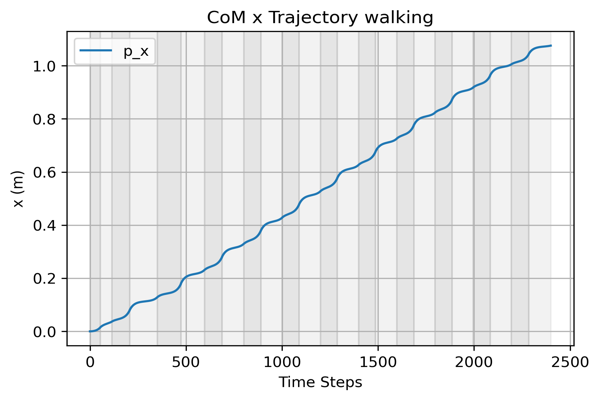
\includegraphics[width=\textwidth]{C:/Users/giuse/OneDrive/Desktop/GITHUB PROJECTS/AMR-FP1/centroidal_dyn-main/plots/CoM x Trajectory walking.png}
        \caption{CoM x component}
        \label{fig:com_x_walking}
    \end{subfigure}
    \hfill
    \begin{subfigure}[b]{0.32\textwidth}
        \centering
        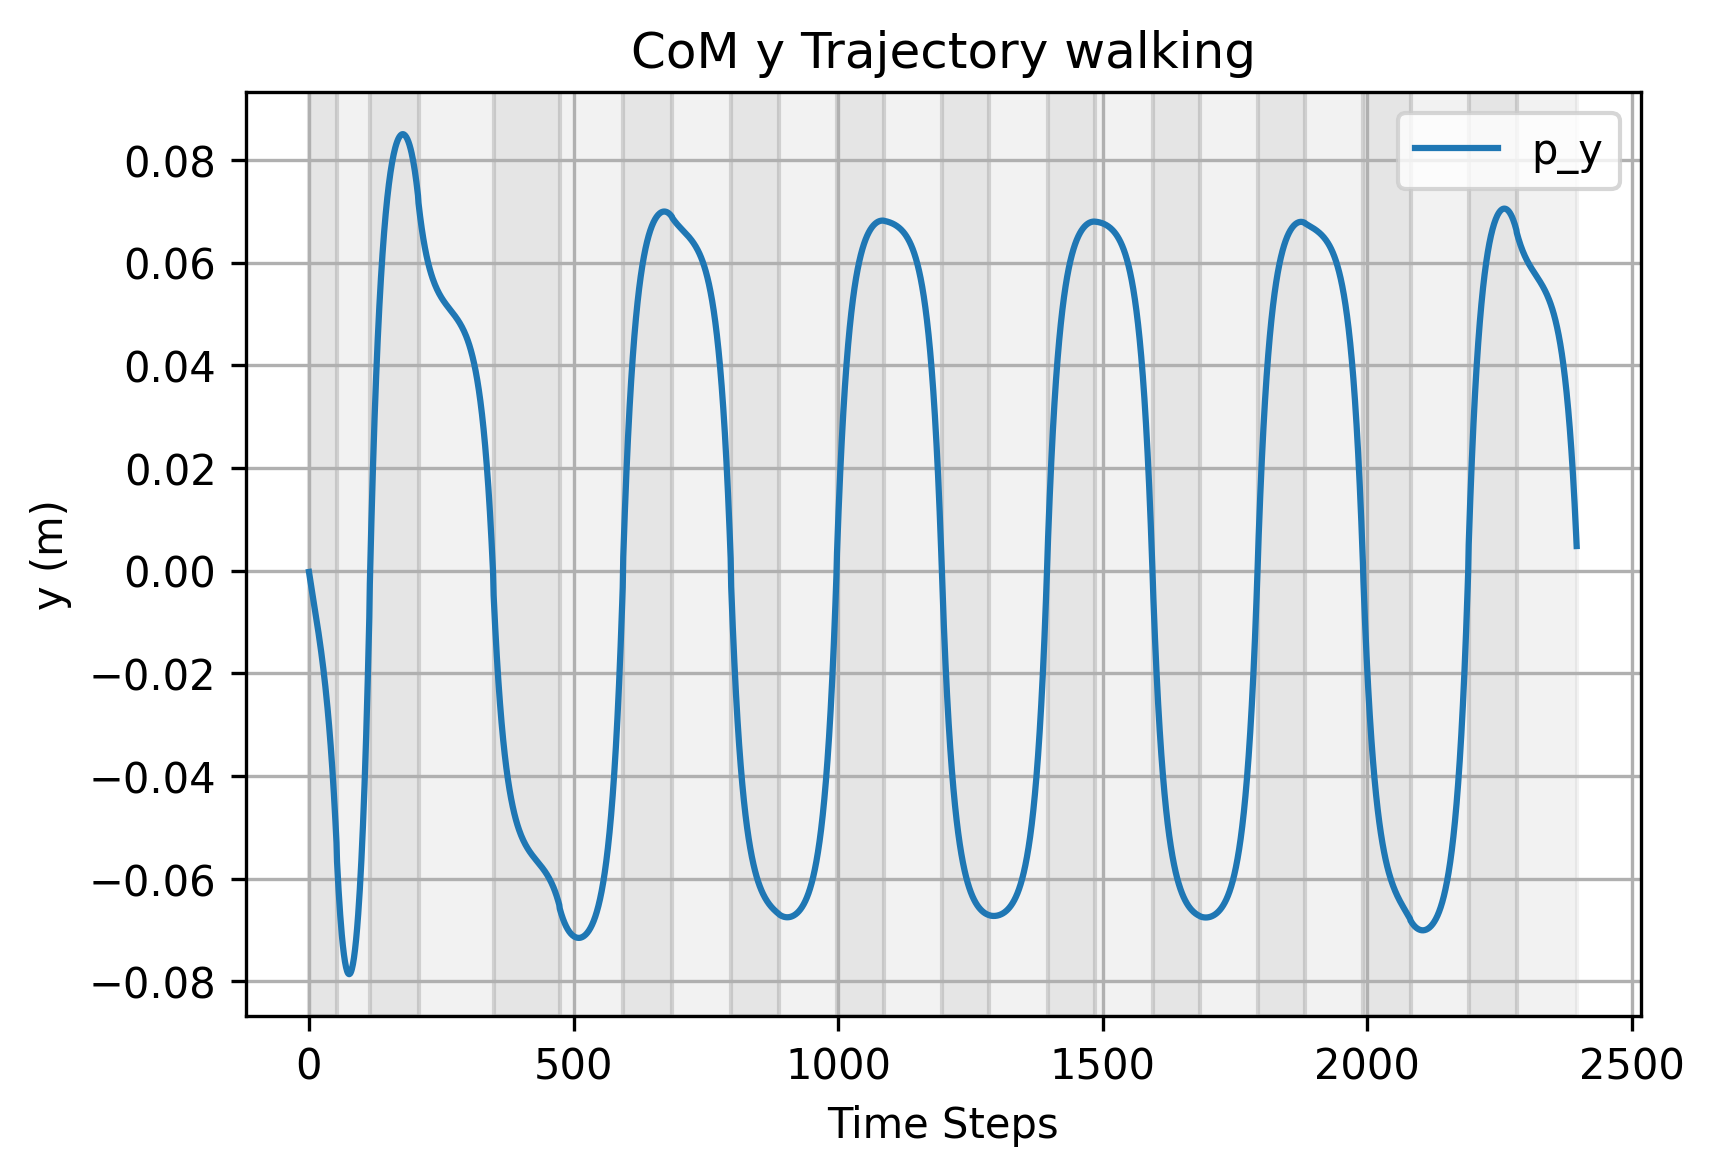
\includegraphics[width=\textwidth]{C:/Users/giuse/OneDrive/Desktop/GITHUB PROJECTS/AMR-FP1/centroidal_dyn-main/plots/CoM y Trajectory walking.png}
        \caption{CoM y component}
        \label{fig:com_y_walking}
    \end{subfigure}
    \hfill
    \begin{subfigure}[b]{0.32\textwidth}
        \centering
        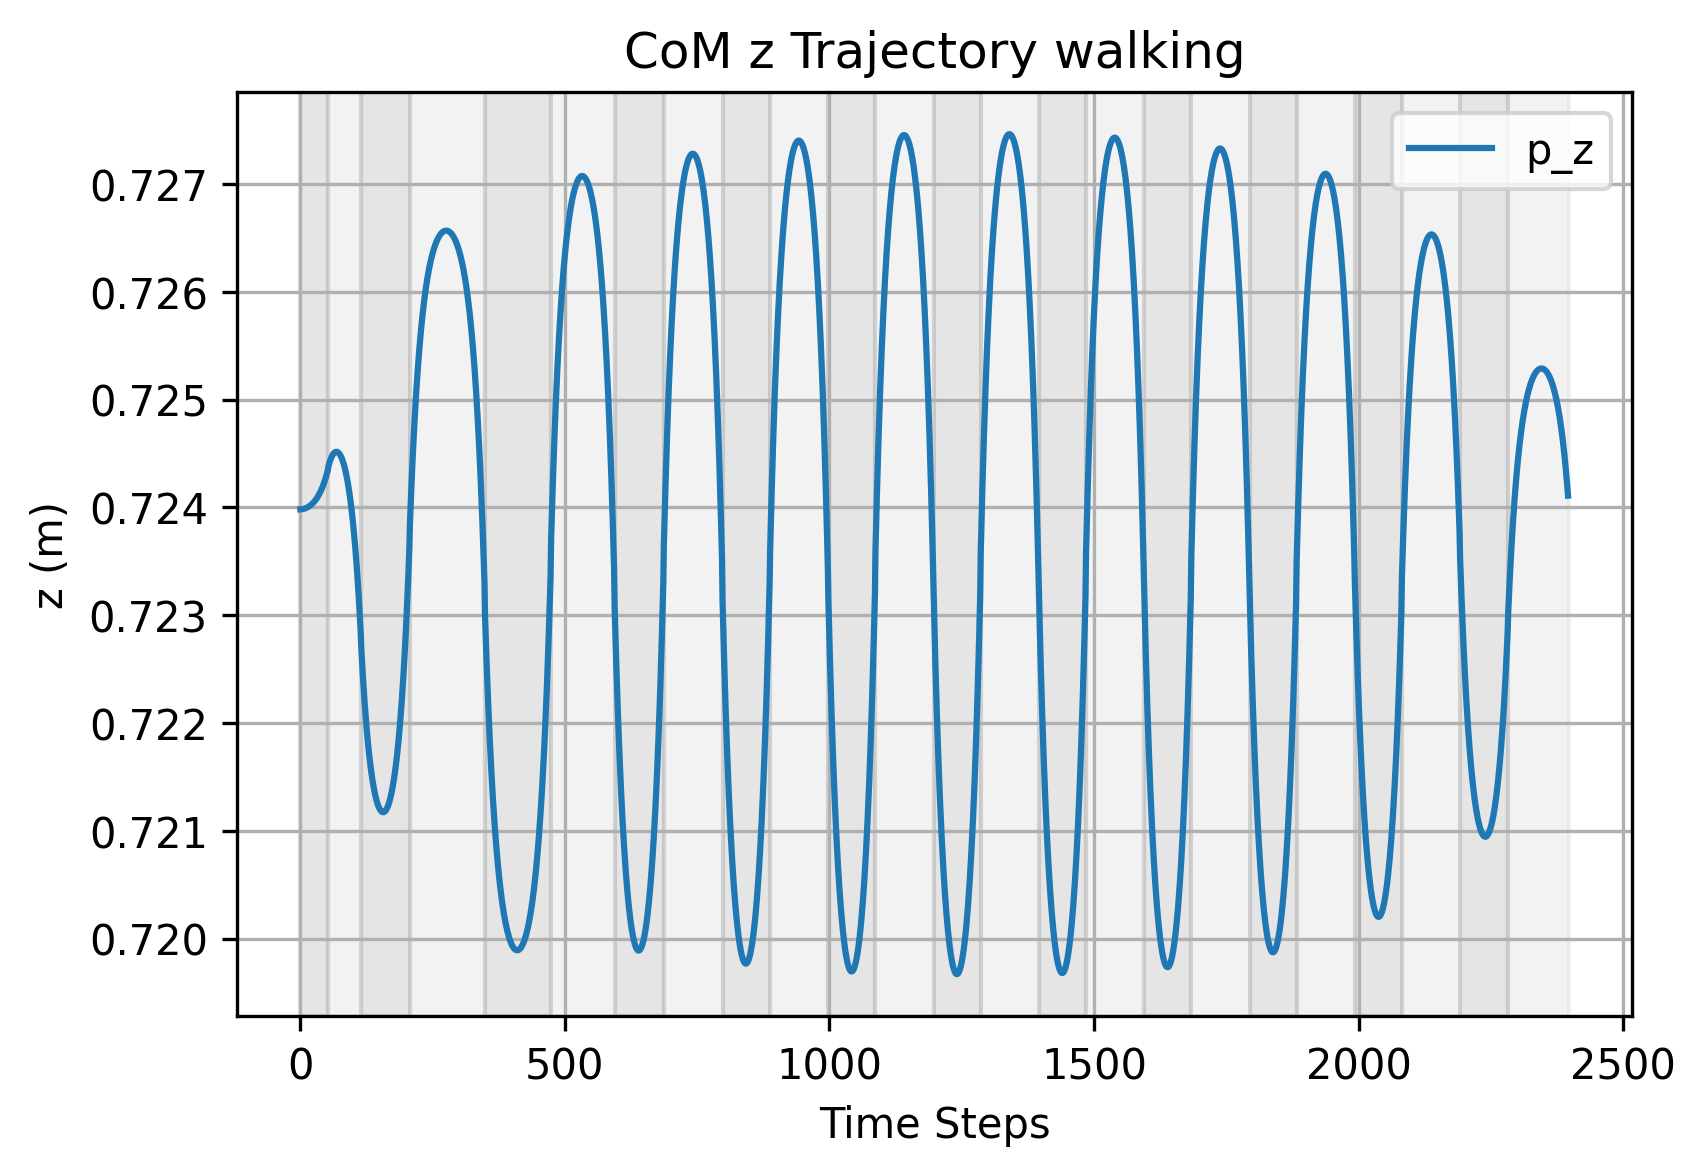
\includegraphics[width=\textwidth]{C:/Users/giuse/OneDrive/Desktop/GITHUB PROJECTS/AMR-FP1/centroidal_dyn-main/plots/CoM z Trajectory walking.png}
        \caption{CoM z component}
        \label{fig:com_z_walking}
    \end{subfigure}
    \caption{Evolution of CoM Position - Walking Task}
    \label{fig:com_walking}
\end{figure}
The plots in Fig. \ref{fig:threeimages_walking} illustrate the dynamics of feet trajectories, CoM velocity, and angular momentum during the walking task. In Fig. \ref{fig:feet_z_walking}, the periodic variations in feet positions along the $z$ axis capture the transition between ground clearance and contact, underscoring the cyclic nature of the walking gait. These fluctuations correspond to the CoM velocity patterns in Fig. \ref{fig:com_velocity_walking}, where oscillations in the $x$ and $y$ components reflect the alternating support phases and weight shifts. In Fig. \ref{fig:angular_momentum_walking}, the angular momentum exhibits pronounced oscillations, particularly in the $x$ component, indicating the corrective torques employed to maintain stability throughout the walking cycle.
\begin{figure}[htbp]
    \centering
    \begin{subfigure}[b]{0.32\textwidth}
        \centering
        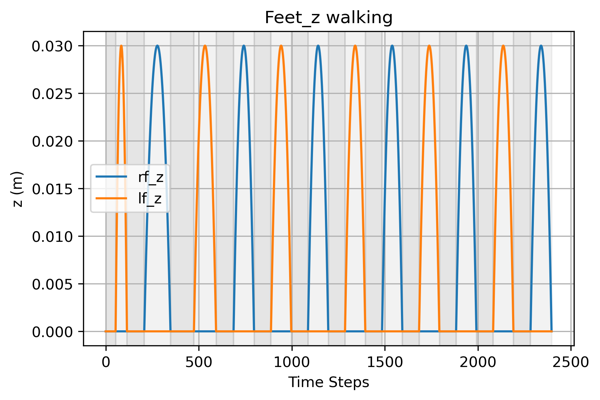
\includegraphics[width=\textwidth]{C:/Users/giuse/OneDrive/Desktop/GITHUB PROJECTS/AMR-FP1/centroidal_dyn-main/plots/Feet_z walking.png}
        \caption{Feet along z axis}
        \label{fig:feet_z_walking}
    \end{subfigure}
    \hfill
    \begin{subfigure}[b]{0.32\textwidth}
        \centering
        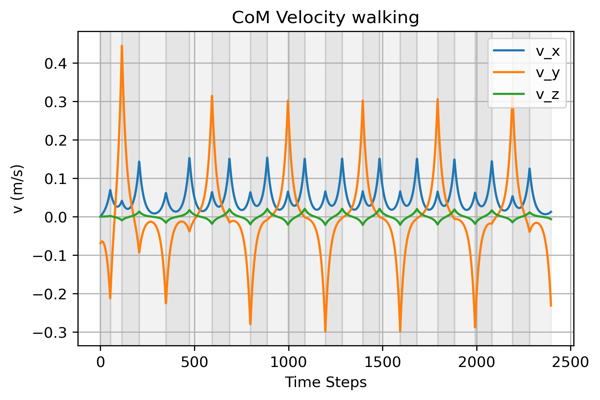
\includegraphics[width=\textwidth]{C:/Users/giuse/OneDrive/Desktop/GITHUB PROJECTS/AMR-FP1/centroidal_dyn-main/plots/CoM Velocity walking.png}
        \caption{CoM Velocity}
        \label{fig:com_velocity_walking}
    \end{subfigure}
    \hfill
    \begin{subfigure}[b]{0.32\textwidth}
        \centering
        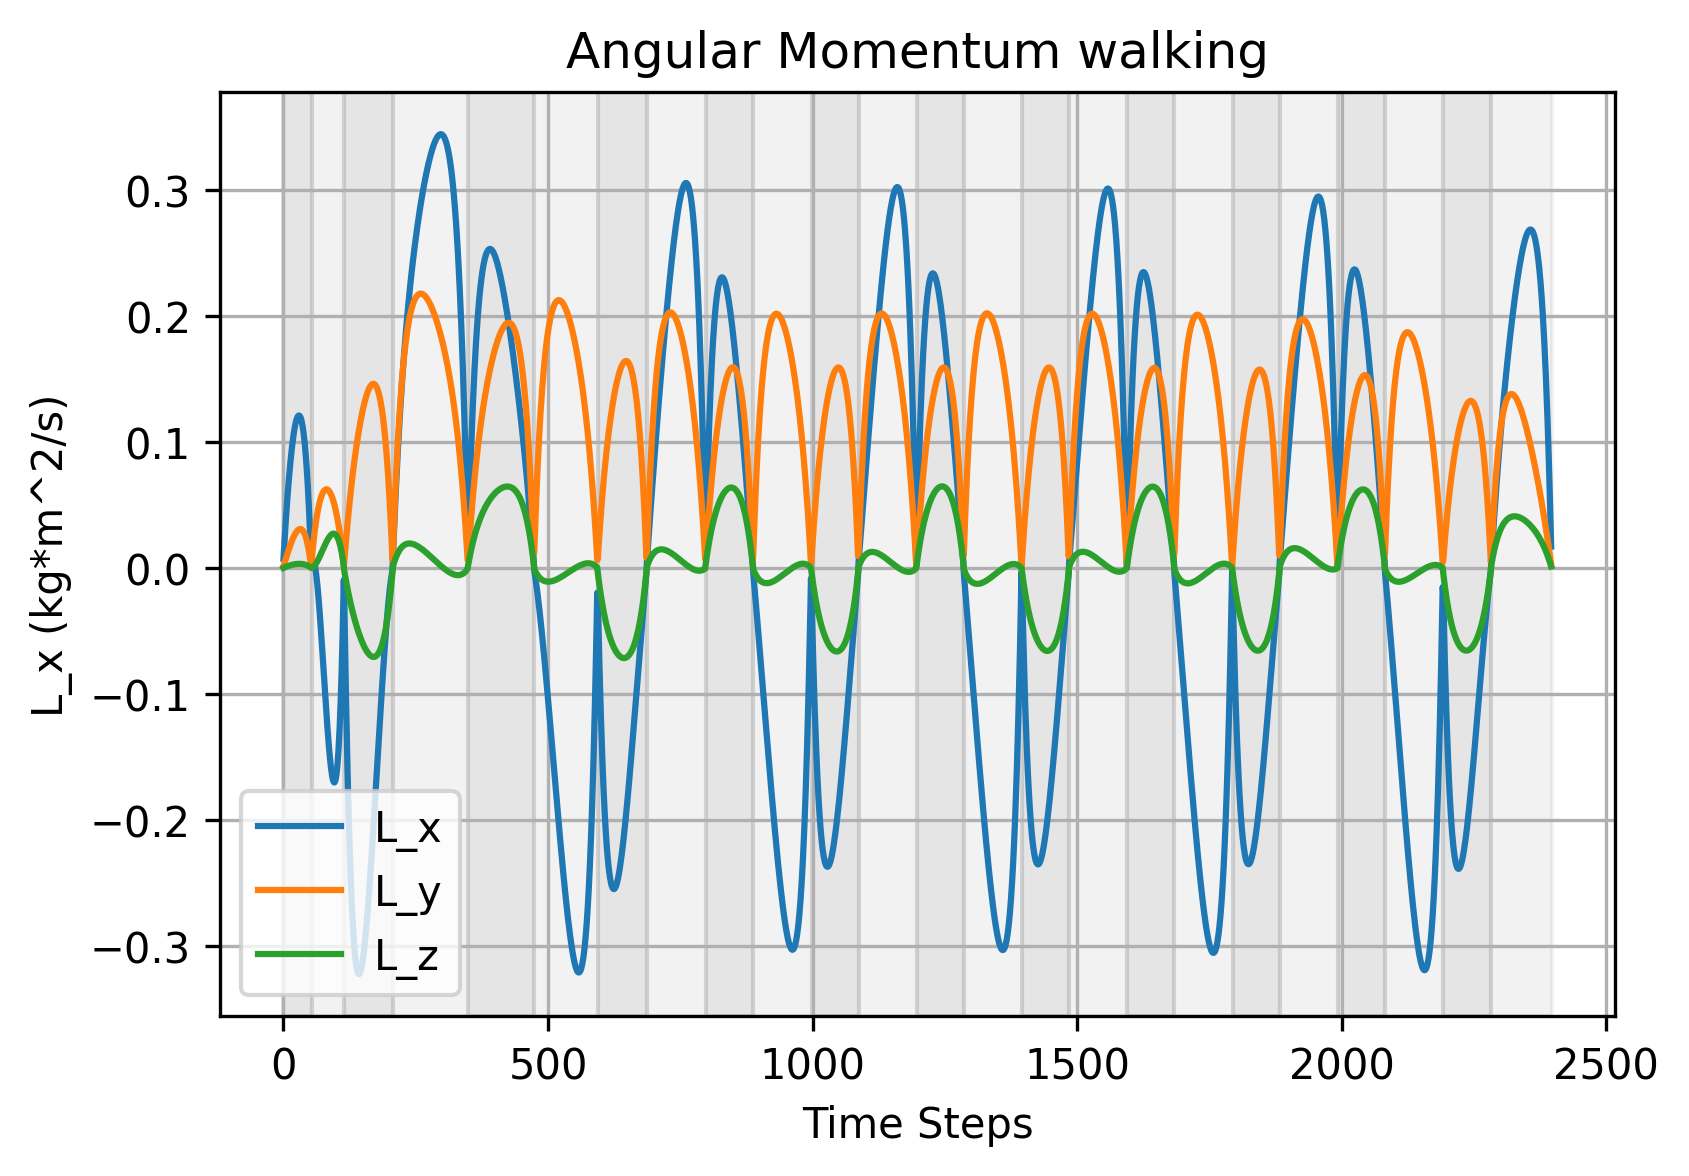
\includegraphics[width=\textwidth]{C:/Users/giuse/OneDrive/Desktop/GITHUB PROJECTS/AMR-FP1/centroidal_dyn-main/plots/Angular Momentum walking.png}
        \caption{Angular Momentum}
        \label{fig:angular_momentum_walking}
    \end{subfigure}
    \caption{Feet, Com Velocity and Angular Momentum - Walking Task}
    \label{fig:threeimages_walking}
\end{figure}
\\
The plots in Fig. \ref{fig:comparison_walking} compare the optimized and reference trajectories for the walking task, highlighting the robot’s adherence to the intended motion patterns. The CoM position plots show a consistent forward motion along the $x$ - axis, lateral oscillations in the $y$ - axis, and minimal vertical fluctuations in the $z$ - axis, indicating stable walking dynamics. CoM velocities reflect these patterns, with pronounced oscillations in the $x$ and $y$ components and minimal $z$ velocity, underscoring vertical stability.
Angular momentum exhibits periodic variations in the $x$ and $y$ components during foot transitions, while the $z$ component remains stable, suggesting controlled rotational behavior. Feet positions and velocity plots capture the cyclic nature of the gait, with distinct lift-off and ground contact phases in the $z$ component and steady forward movement in the $x$ component. Overall, the optimized trajectories align well with the reference paths, with minor adjustments indicating corrective actions for stability.
\begin{figure}[htbp]
    \centering
    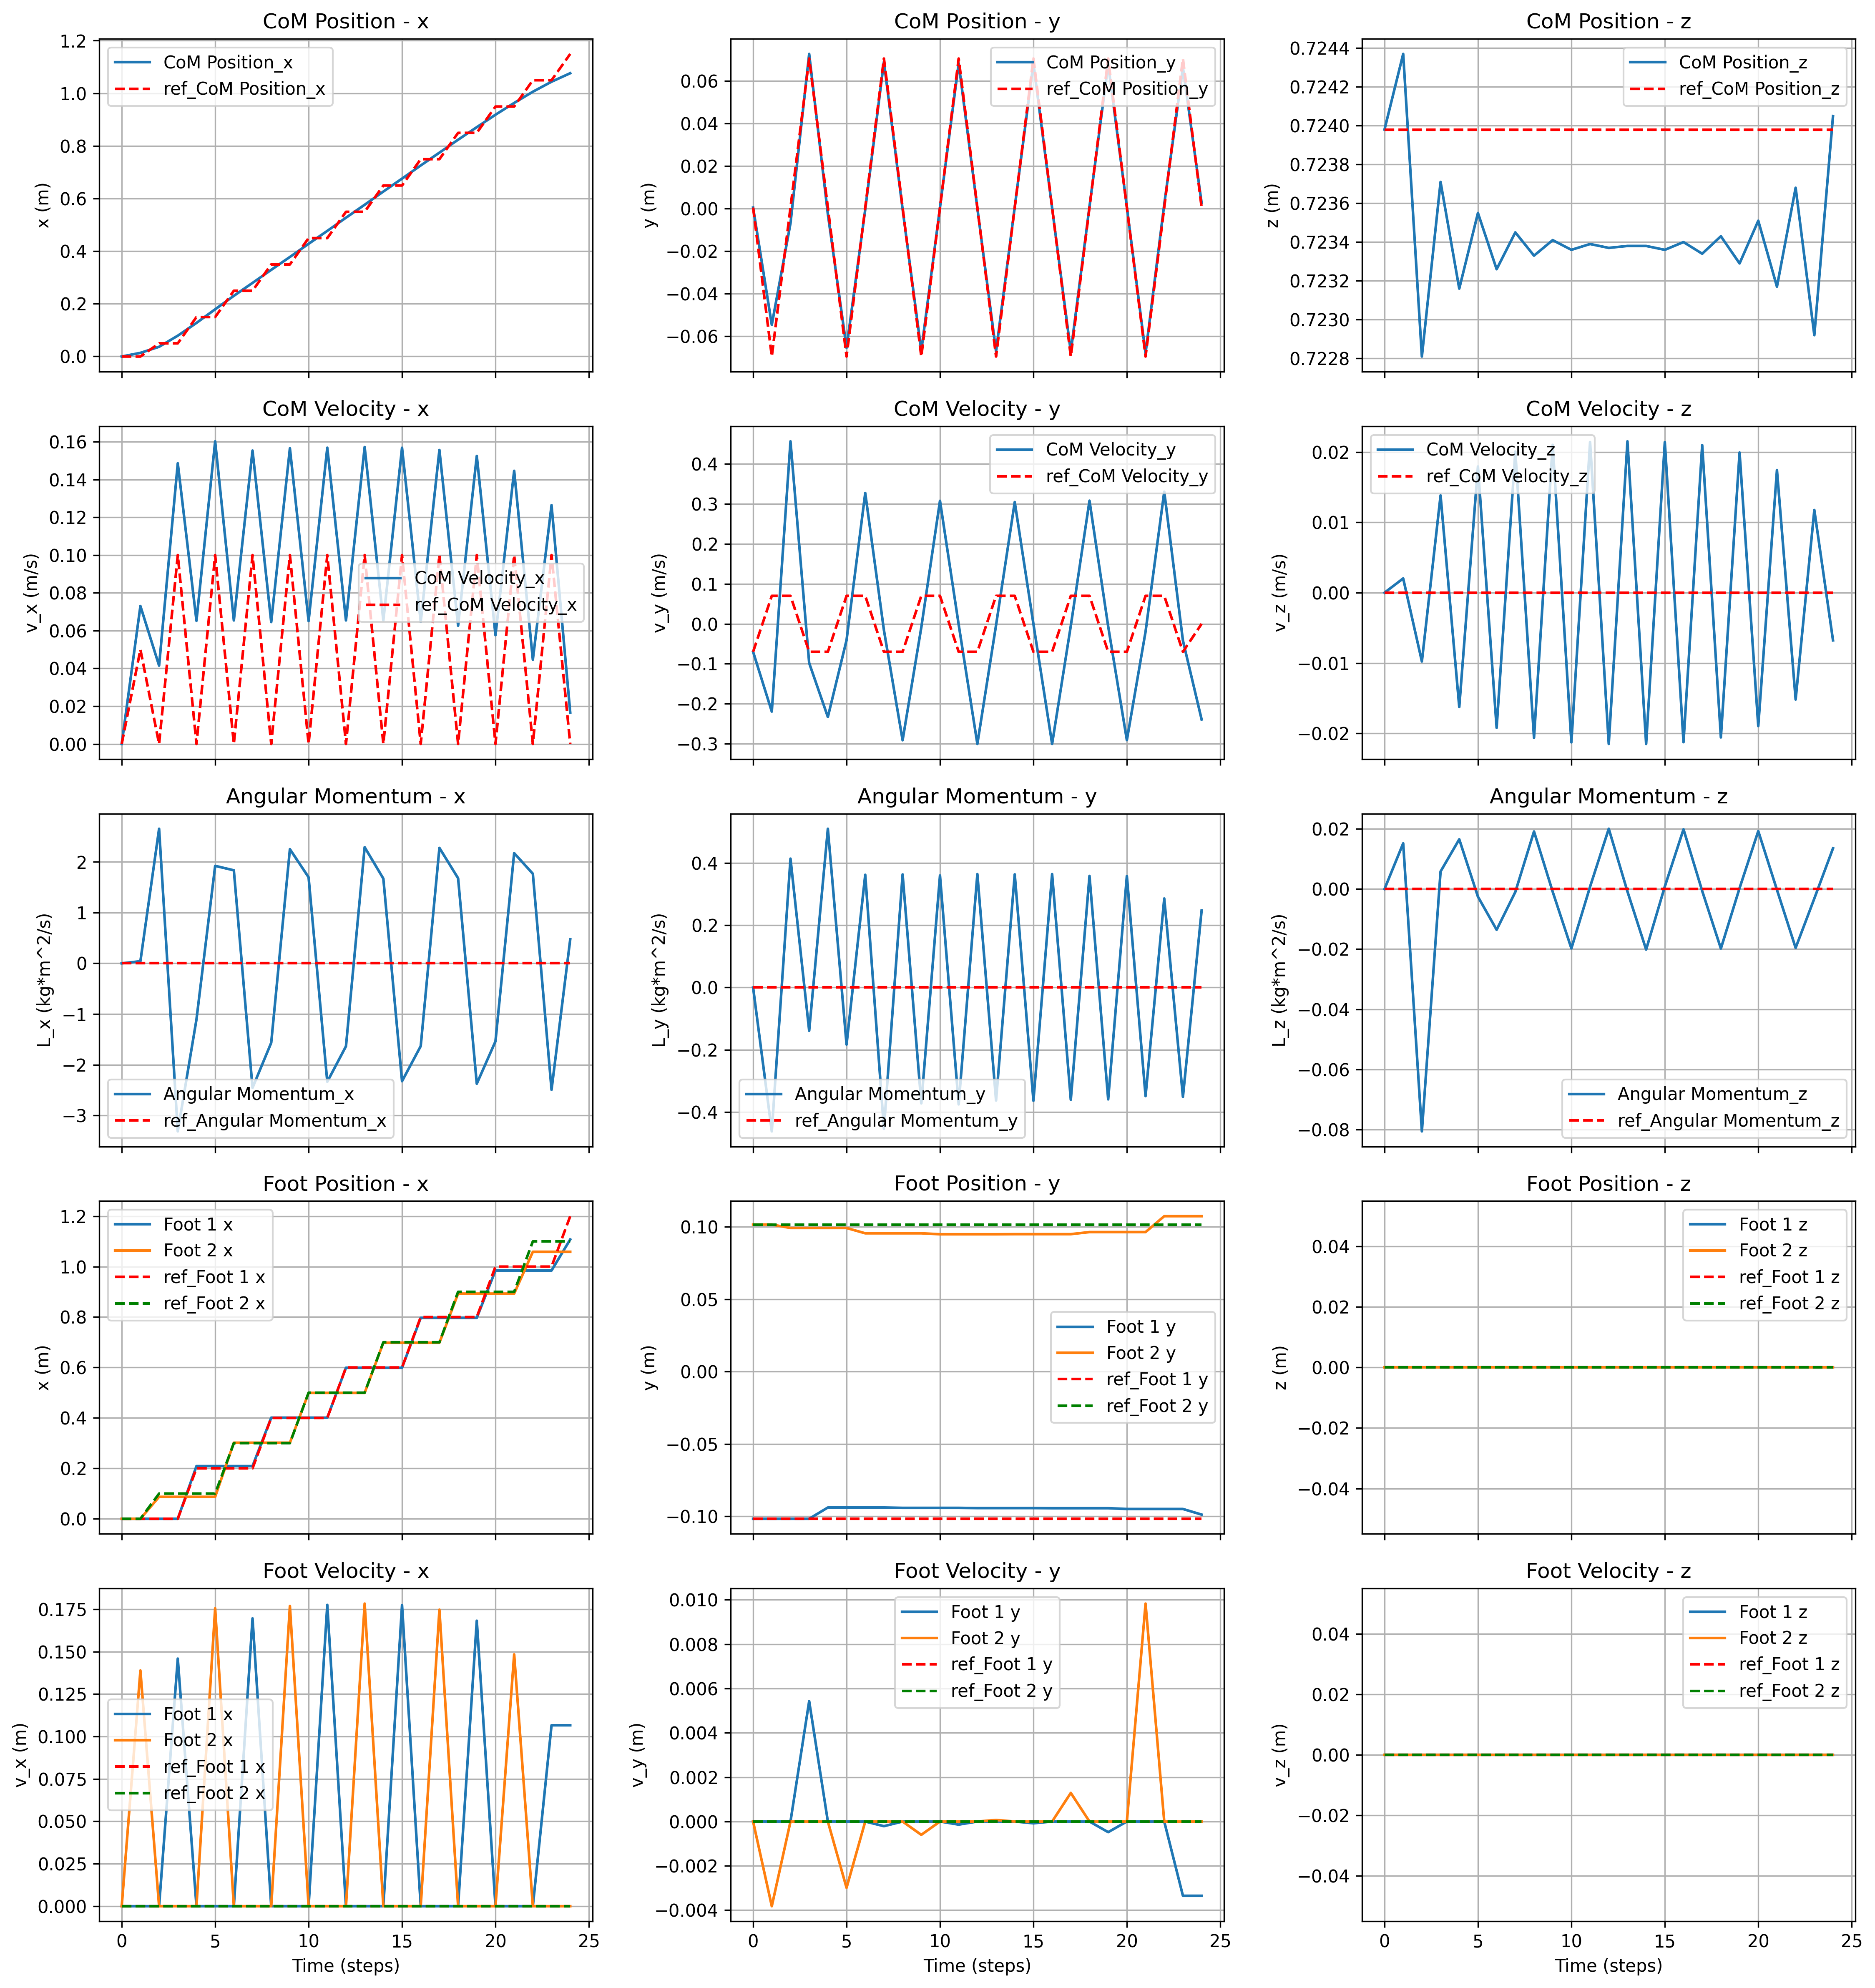
\includegraphics[width=0.8\textwidth]{C:/Users/giuse/OneDrive/Desktop/GITHUB PROJECTS/AMR-FP1/centroidal_dyn-main/plots/contact_x_walking.png}
    \caption{Trajectory vs Reference - Walking Task}
    \label{fig:comparison_walking}
\end{figure}
\newpage
As for the still task, the analysis of the contact forces during the walking task is crucial to verify that the robot maintains balance while executing the motion. As shown in Table \ref{tab:forces_walking}, the sum of the contact forces along the $z$-axis consistently aligns with the gravitational force acting on the robot. This alignment indicates that the control strategy effectively regulates vertical support forces, ensuring stability throughout the gait sequence.
\begin{table}[H]
    \centering
    \renewcommand{\arraystretch}{1.2}
    \resizebox{\textwidth}{!}{
        \begin{tabular}{c|c|c|c|c}
            \hline
            Interval & Right Foot (x,y,z) & Left Foot (x,y,z) & $\Sigma L_k$ & Sum Forces (x,y,z) \\
            \hline
            0 & (0.3098, 10.0006, 49.0692) & (0.3076, -8.8127, 49.0480) & (0, 0) & (0.6174, 1.1878, 98.1172) \\
            1 & (-2.9107, 12.2335, 97.9563) & (0, 0, 0) & (0, -1) & (-2.9107, 12.2335, 97.9563) \\
            2 & (3.2811, -0.3468, 48.5795) & (-4.8871, -19.6105, 49.9662) & (0, 0) & (-1.6060, -19.9572, 98.5457) \\
            3 & (0, 0, 0) & (-6.4470, 4.1862, 97.4919) & (-1, 0) & (-6.4470, 4.1862, 97.4919) \\
            4 & (-6.8093, 14.0802, 49.7681) & (4.0998, -3.9816, 49.0385) & (0, 0) & (-2.7095, 10.0986, 98.8066) \\
            5 & (-6.9116, 1.8871, 97.3107) & (0, 0, 0) & (0, -1) & (-6.9116, 1.8871, 97.3107) \\
            6 & (3.1803, 1.8069, 49.0314) & (-5.8173, -15.9695, 49.9272) & (0, 0) & (-2.6370, -14.1626, 98.9586) \\
            7 & (0, 0, 0) & (-6.7673, 0.4847, 97.2130) & (-1, 0) & (-6.7673, 0.4847, 97.2130) \\
            8 & (-5.9977, 15.1901, 49.9258) & (3.4081, -2.5941, 49.0988) & (0, 0) & (-2.5896, 12.5961, 99.0246) \\
            9 & (-6.7991, 0.5855, 97.1717) & (0, 0, 0) & (0, -1) & (-6.7991, 0.5855, 97.1717) \\
            10 & (3.3447, 2.2144, 49.0962) & (-5.9424, -15.5259, 49.9575) & (0, 0) & (-2.5977, -13.3115, 99.0537) \\
            11 & (0, 0, 0) & (-6.7993, -0.1305, 97.1539) & (-1, 0) & (-6.7993, -0.1305, 97.1539) \\
            12 & (-5.9816, 15.3748, 49.9533) & (3.3785, -2.3771, 49.1101) & (0, 0) & (-2.6031, 12.9977, 99.0634) \\
            13 & (-6.8083, 0.3513, 97.1498) & (0, 0, 0) & (0, -1) & (-6.8083, 0.3513, 97.1498) \\
            14 & (3.3689, 2.2945, 49.1029) & (-5.9736, -15.4697, 49.9601) & (0, 0) & (-2.6047, -13.1752, 99.0630) \\
            15 & (0, 0, 0) & (-6.8037, -0.1903, 97.1550) & (-1, 0) & (-6.8037, -0.1903, 97.1550) \\
            16 & (-5.9649, 15.3831, 49.9465) & (3.3681, -2.3898, 49.1053) & (0, 0) & (-2.5968, 12.9933, 99.0517) \\
            17 & (-6.7893, 0.4215, 97.1738) & (0, 0, 0) & (0, -1) & (-6.7893, 0.4215, 97.1738) \\
            18 & (3.3633, 2.2973, 49.0756) & (-5.9344, -15.6231, 49.9448) & (0, 0) & (-2.5711, -13.3258, 99.0204) \\
            19 & (0, 0, 0) & (-6.7306, 0.0657, 97.2207) & (-1, 0) & (-6.7306, 0.0657, 97.2207) \\
            20 & (-5.8564, 15.2809, 49.8788) & (3.3748, -2.7034, 49.0690) & (0, 0) & (-2.4816, 12.5775, 98.9477) \\
            21 & (-6.5267, 1.0544, 97.3302) & (0, 0, 0) & (0, -1) & (-6.5267, 1.0544, 97.3302) \\
            22 & (3.5736, 2.3792, 48.9388) & (-5.7275, -16.6990, 49.8343) & (0, 0) & (-2.1539, -14.3198, 98.7732) \\
            23 & (0, 0, 0) & (-5.5944, 1.6324, 97.5852) & (-1, 0) & (-5.5944, 1.6324, 97.5852) \\
            \hline
        \end{tabular}
    }
    \caption{Summary of Forces and Foot Positions per Interval - Walking Task}
    \label{tab:forces_walking}
\end{table}    
To conclude the analysis of the walking task, Figures \ref{fig:contact_forces_walking_right} and \ref{fig:contact_forces_walking_left} depict the behavior of the translational and rotational forces at the contact points for the right and left foot, respectively. Along the horizontal axes, the translational forces exhibit periodic fluctuations, corresponding to the alternating support phases during the walking cycle. In the vertical direction ( $z$ - axis), the forces consistently counteract gravitational effects, with pronounced peaks reflecting ground contact phases and troughs indicating foot lift-off events.
Rotational forces show notable oscillations in both the $x$ and $y$ components, particularly during transitions between single and double support phases, indicating the corrective torques applied to maintain balance. The $z$ component remains relatively stable, with minor oscillations that align with the angular momentum patterns previously observed.
\begin{figure}[htbp]
    \centering
    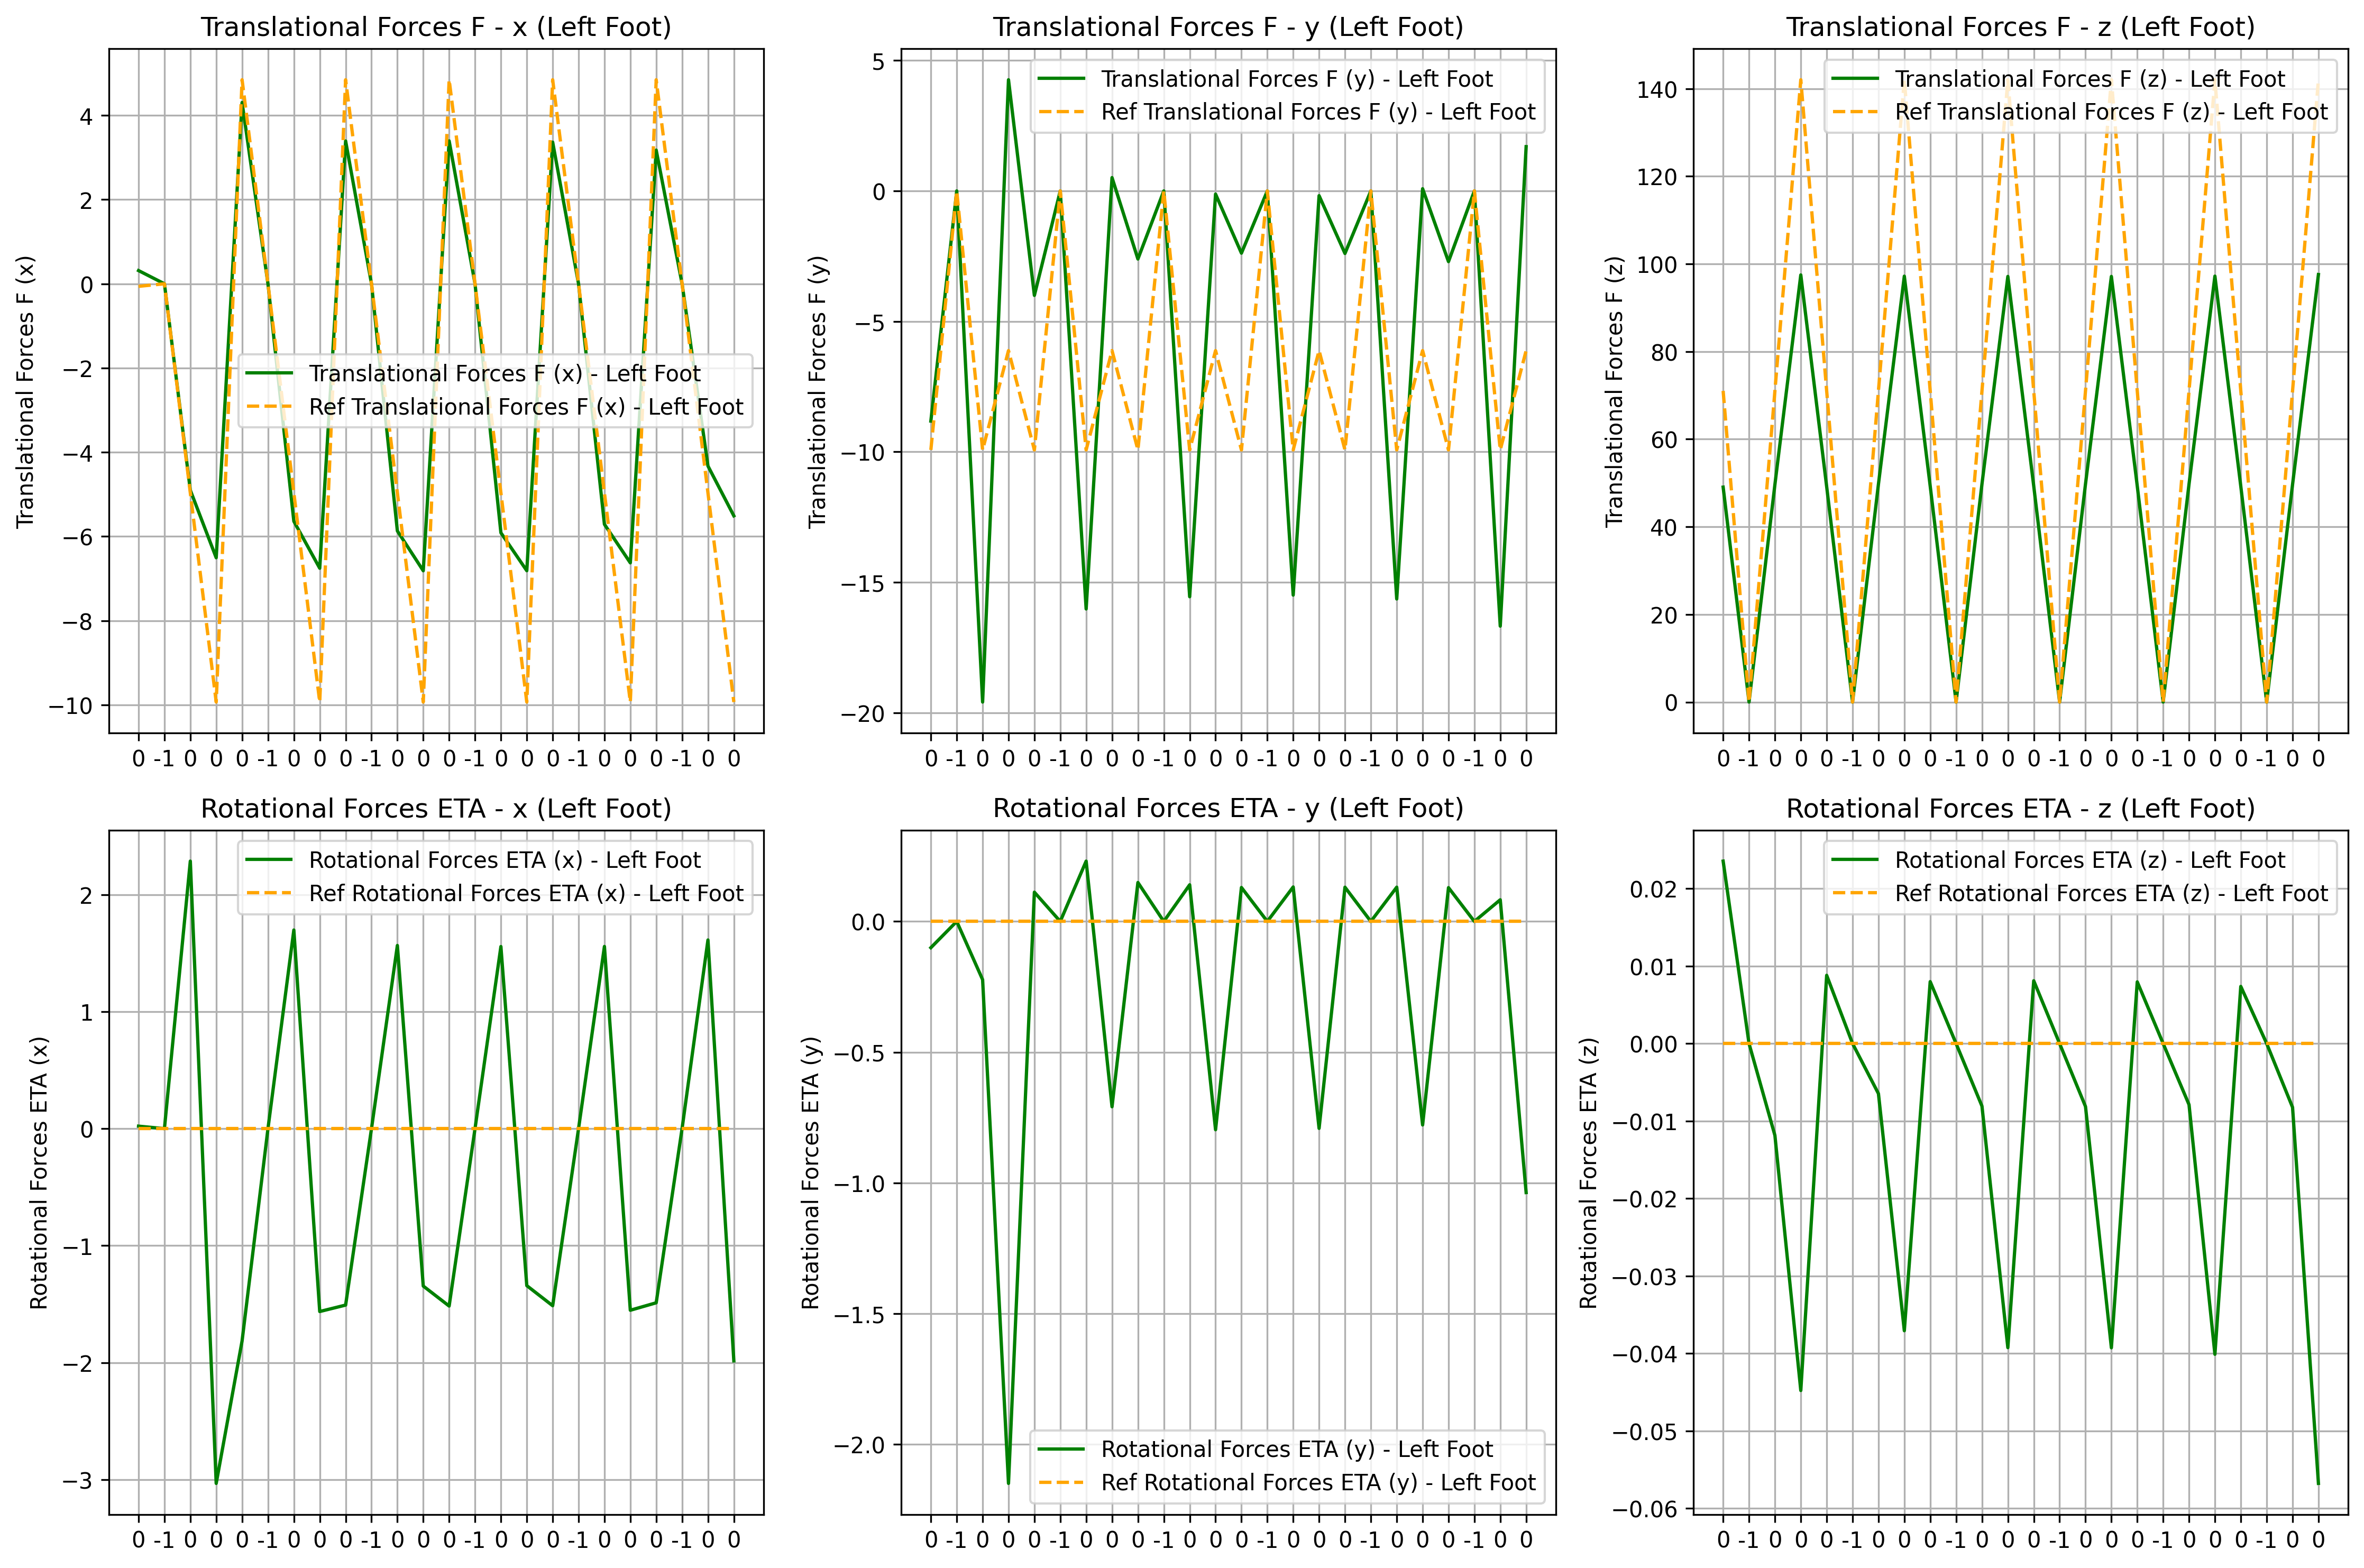
\includegraphics[width=0.8\textwidth]{C:/Users/giuse/OneDrive/Desktop/GITHUB PROJECTS/AMR-FP1/centroidal_dyn-main/plots/contact_forces_walking_right.png}
    \caption{Translational and Rotational Forces Right Foot - Walking Task}
    \label{fig:contact_forces_walking_right}
    
    \vspace{1em} % Adjusts the space between the two plots

    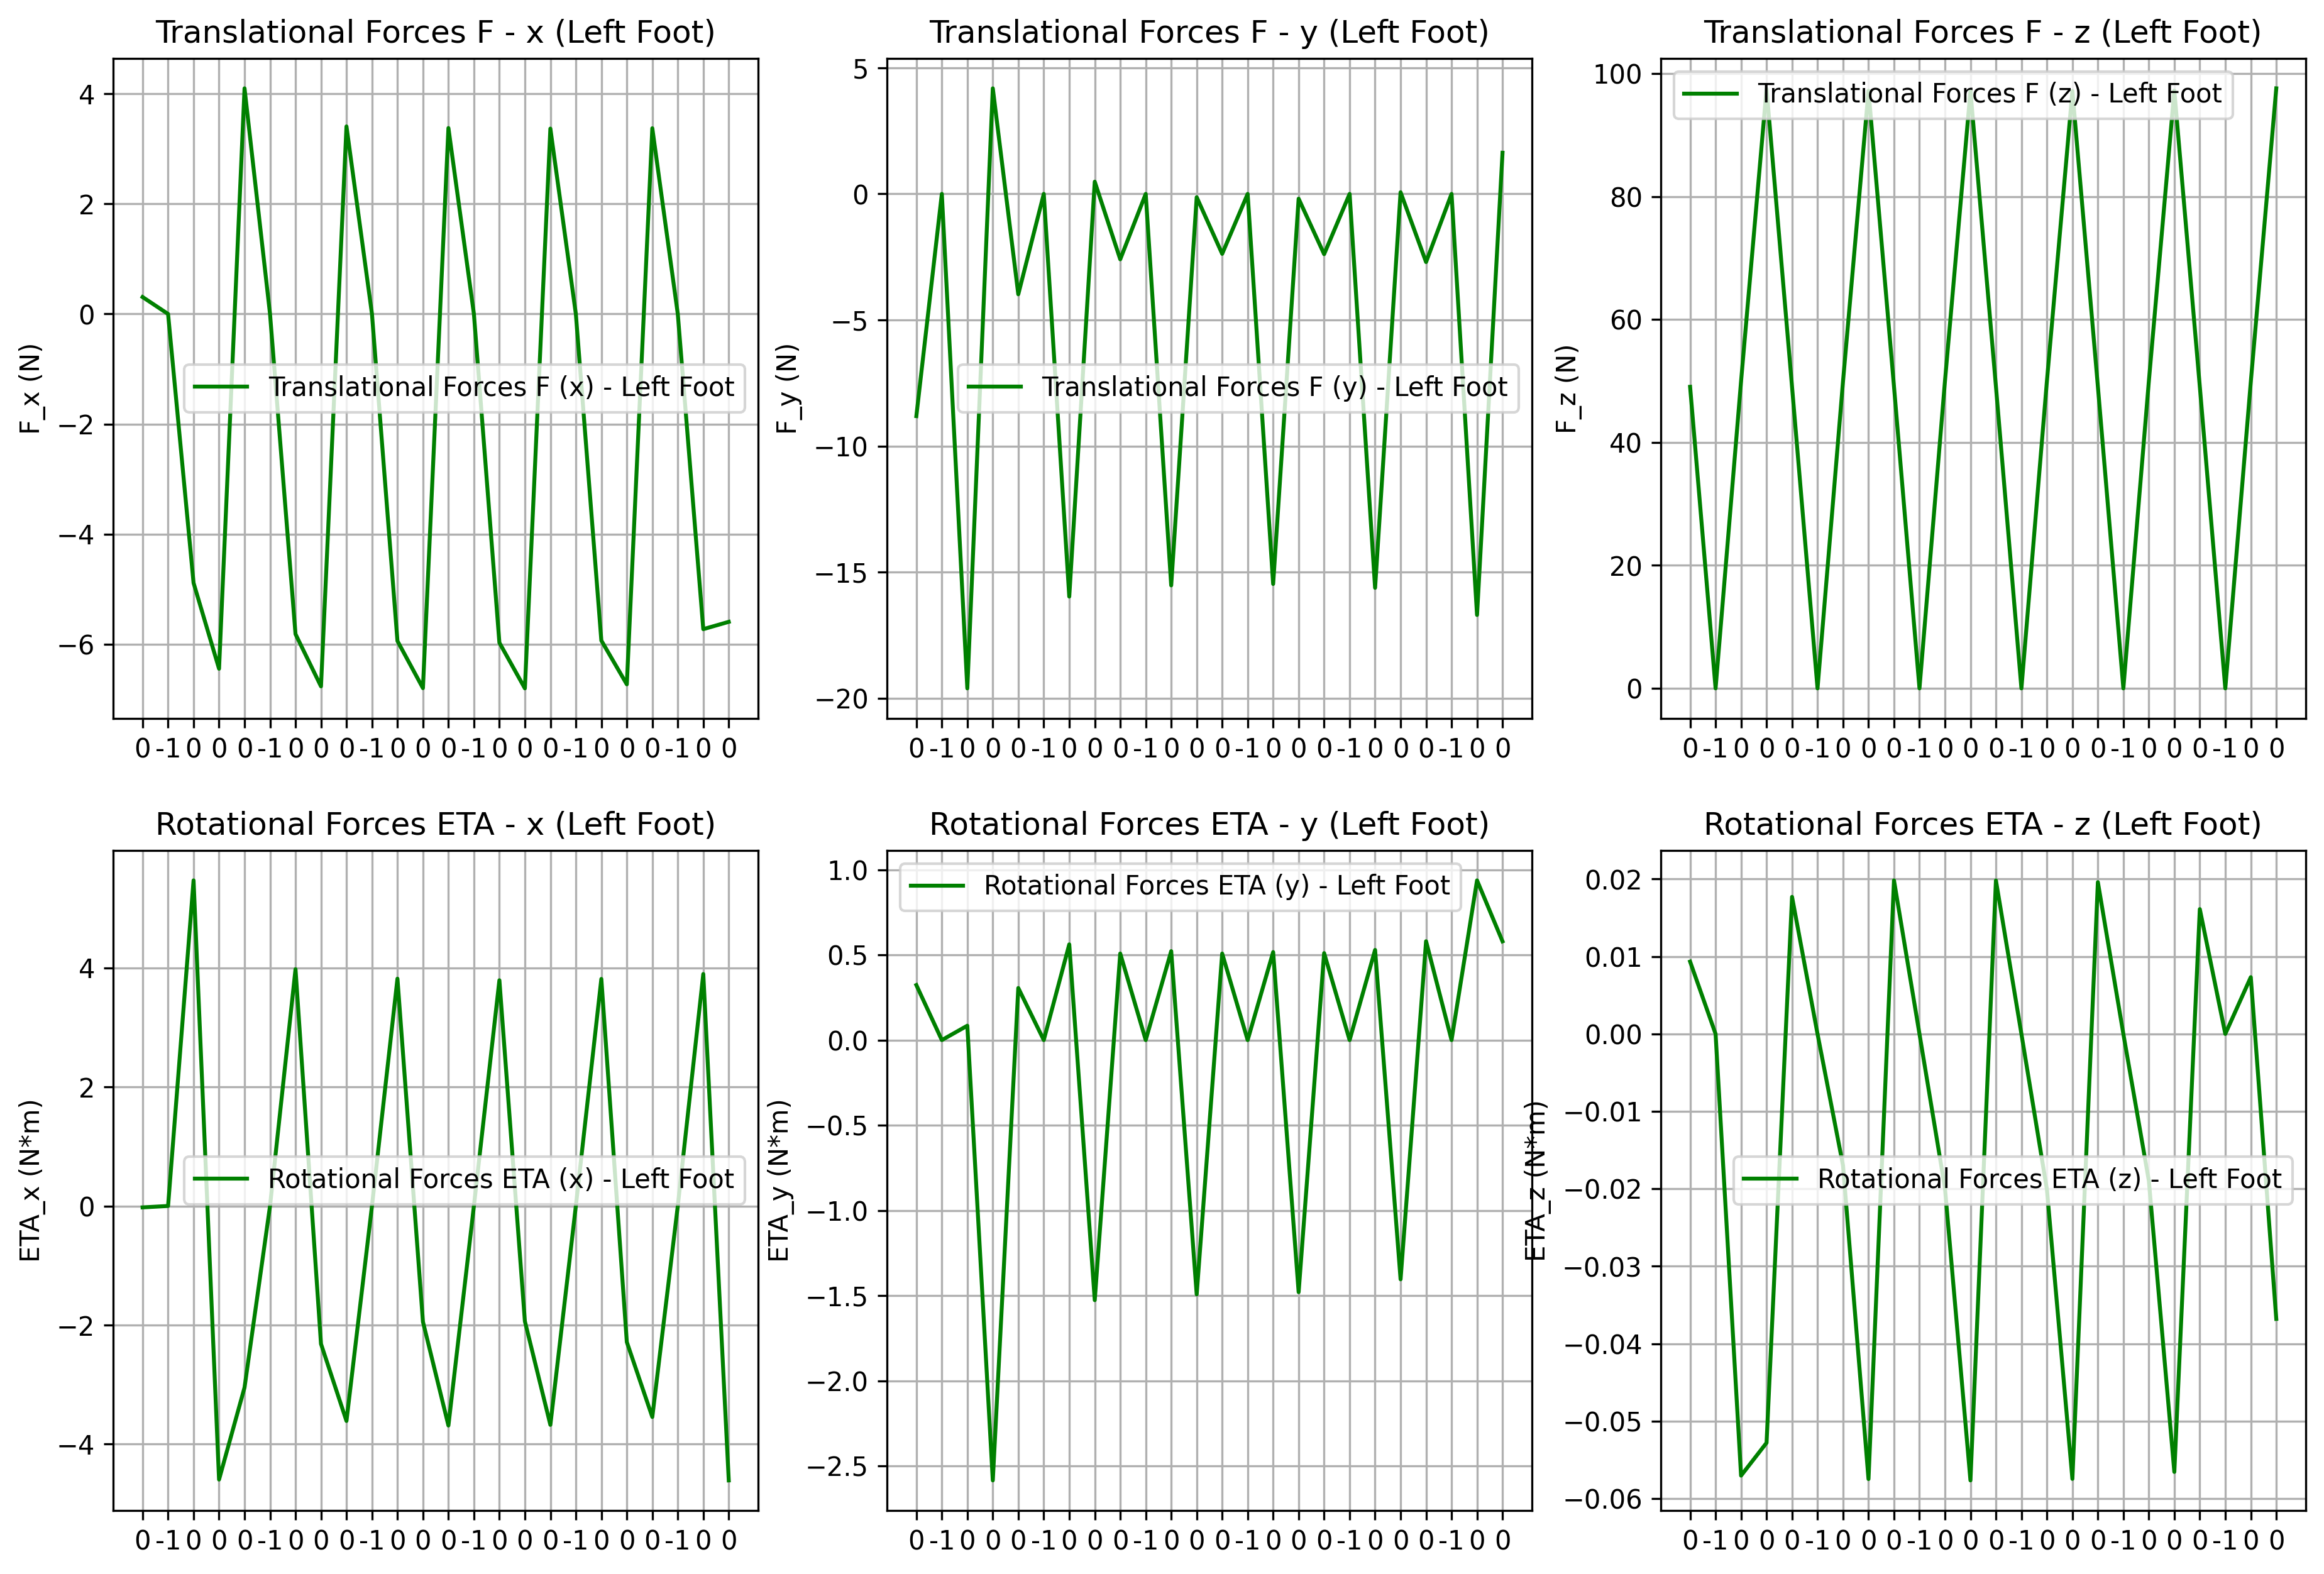
\includegraphics[width=0.8\textwidth]{C:/Users/giuse/OneDrive/Desktop/GITHUB PROJECTS/AMR-FP1/centroidal_dyn-main/plots/contact_forces_walking_left.png}
    \caption{Translational and Rotational Forces Left Foot - Walking Task}
    \label{fig:contact_forces_walking_left}
\end{figure}
\end{sloppypar}

\end{document}